\documentclass[12pt]{book}
\usepackage[utf8]{inputenc}
\usepackage{multirow}
\usepackage{listings}
\usepackage{amssymb,amsmath,amsthm,amsfonts}
\usepackage{calc}
\usepackage{graphicx}
\usepackage{subfigure}
\usepackage{indentfirst}
\usepackage{titlesec}
%\newcommand{\sectionbreak}{\clearpage}
\DeclareGraphicsExtensions{.bmp,.png,.pdf,.jpg}
\usepackage{textcomp, gensymb}
\usepackage{url}
\usepackage{amsmath}
\usepackage{graphicx}
\graphicspath{{images/}}
\usepackage{parskip}
\usepackage{fancyhdr}
\usepackage{vmargin}
\setmarginsrb{2 cm}{2 cm}{2 cm}{2 cm}{1 cm}{1.5 cm}{1 cm}{1.5 cm}

\usepackage[spanish]{babel}
\usepackage[colorlinks=true, allcolors=blue]{hyperref}
\hypersetup{
    colorlinks=true,% make the links colored
}
\usepackage[nolist]{acronym}
\usepackage[table]{xcolor}
\usepackage{url}

% \boxed no tolera los endline
\newcommand\mybox[2][l]{\fbox{\begin{tabular}{@{}#1@{}}#2\end{tabular}}}

%% Biblatex
% \usepackage[style=plain]{biblatex}
% \addbibresource{bibliografia.bib}


\lstdefinelanguage{Marlowe}{%
  language     = Haskell,
  morekeywords = {Close, Pay, Assert, If, When, Let},
}
\lstdefinelanguage{Isabelle}{%
  language     = ML,
  morekeywords = {theory, imports, begin, end},
}

\definecolor{codegreen}{rgb}{0,0.6,0}
\definecolor{codegray}{rgb}{0.5,0.5,0.5}
\definecolor{codepurple}{rgb}{0.58,0,0.82}
\definecolor{backcolour}{rgb}{0.95,0.95,0.92}

\lstdefinestyle{Haskell-cardano}{
    backgroundcolor=\color{backcolour},   
    commentstyle=\color{codegreen},
    keywordstyle=\color{magenta},
    numberstyle=\tiny\color{codegray},
    stringstyle=\color{codepurple},
    basicstyle=\ttfamily\footnotesize,
    breakatwhitespace=false,         
    language=Haskell,
    breaklines=true,                 
    captionpos=b,                    
    keepspaces=true,                 
    numbers=none,                    
    numbersep=5pt,                  
    showspaces=false,                
    showstringspaces=false,
    showtabs=false,                  
    tabsize=2
}

\definecolor{isarblue}{HTML}{006699}
\definecolor{isargreen}{HTML}{009966}
\lstdefinelanguage{isabelle}{%
    keywords=[1]{type_synonym,datatype,fun,abbreviation,definition,proof,lemma,theorem, theory,corollary},
    keywordstyle=[1]\bfseries\color{isarblue},
    keywords=[2]{where,assumes,shows,and, imports, begin, end},
    keywordstyle=[2]\bfseries\color{isargreen},
    keywords=[3]{if,then,else,case,of,SOME,let,in,O},
    keywordstyle=[3]\color{isarblue},
}
\lstdefinestyle{Isabelle}{%
  language=isabelle,
  escapeinside={&}{&},
  columns=fixed,
  extendedchars,
  frame=single,
  basewidth={0.5em,0.45em},
  basicstyle=\ttfamily,
  mathescape,
}

% \documentclass[9pt,oneside]{amsart}
\usepackage{multicol}
% \usepackage[a4paper,
%             width=170mm,
%             top=18mm,
%             bottom=22mm,
%             includeheadfoot]{geometry}
% \usepackage[bookmarks=true,
%             unicode=true,
%             pdftitle={ACTUS Technical Specification},
%             pdfauthor={ACTUS Financial Research Foundation},
%             pdfkeywords={ACTUS, Financial Contracts, Algorithmic Contracts, Technical Specification},
%             pdfborder={0 0 0.5 [1 3]}]{hyperref}

% ---------------------- floats ----------------------
\usepackage{graphicx}
\usepackage{float}
\usepackage{longtable}

% ---------------------- math ----------------------
\usepackage{amsmath}
\usepackage{amssymb}
\usepackage{amsthm}
\newtheorem{example}{Example}

% ---------------------- custom tables ----------------------
\newenvironment{states}[1]{
	\hfill % force subsection before longtable
	\begin{longtable}{| p{0.05\textwidth} | p{0.48\textwidth} |  p{0.43\textwidth} |}
	\multicolumn{3}{c}{\textbf{#1: State Variables Initialization}}\\ \hline
	\textbf{State} & \textbf{Initialization per $t_0$} & \textbf{Comments} \\
	\hline
	\endfirsthead
	\multicolumn{3}{c}{\textit{Continúa desde la página anterior}} \\
	\hline
	\textbf{State} & \textbf{Initialization per $t_0$} & \textbf{Comments} \\
	\hline
	\endhead
	\hline \multicolumn{3}{r}{\textit{Continúa en la siguiente página}} \\
	\endfoot
	\endlastfoot
}{%
	\hline
	\end{longtable}
}

\newenvironment{schedule}[1]{
	\hfill % force subsection before longtable
	\begin{longtable}{| p{0.05\textwidth} | p{0.5\textwidth} |  p{0.4\textwidth} |}
	\multicolumn{3}{c}{\textbf{#1: Contract Schedule}}\\
	\hline
	\textbf{Event} & \textbf{Schedule} & \textbf{Comments} \\
	\hline
	\endfirsthead
	\multicolumn{2}{c}{\textit{Continua desde la página anterior}} \\
	\hline
	\textbf{Event} & \textbf{Schedule} & \textbf{Comments} \\
	\hline
	\endhead
	\hline \multicolumn{2}{r}{\textit{Continua en la siguiente página}} \\
	\endfoot
	\endlastfoot
}{%
	\hline 
	\end{longtable}
}

\newenvironment{functions}[1]{
	\hfill % force subsection before longtable
    	\begin{longtable}{| p{0.05\textwidth} | p{0.42\textwidth} |  p{0.48\textwidth} |}
	\multicolumn{3}{c}{\textbf{#1: State Transition Functions and Payoff Functions}}\\
	\hline
	\textbf{Event} & \textbf{Payoff Function} & \textbf{State Transition Function}\\
	\hline
	\endfirsthead
	\multicolumn{2}{c}{\textit{Continua desde la página anterior}} \\
	\hline
	\textbf{Event} & \textbf{Payoff Function} & \textbf{State Transition Function}\\
	\hline
	\endhead
	\hline \multicolumn{2}{r}{\textit{Continua en la siguiente página}} \\
	\endfoot
	\endlastfoot
}{%
	\hline
        \end{longtable}
}


% ---------------------- custom notation ----------------------
\newcommand{\Real}{\mathbb{R}}
\newcommand{\Nat}{\mathbb{N}}
\newcommand{\svar}[2]{\textbf{#1}_{#2}}
\newcommand{\attr}[1]{\texttt{#1}}
\newcommand{\stf}[2]{STF\_#1\_#2()}
\newcommand{\pof}[2]{POF\_#1\_#2()}
\newcommand{\dfl}[1]{D (\textbf{Prf}_{#1})}
\newcommand{\sgn}{R (\attr{CNTRL})}
\newcommand{\sdl}[3]{S (#1,#2,#3)}
\newcommand{\sdll}[4]{S (#1,#2,#3,#4)}
\newcommand{\vsdl}[3]{\vec{S} (#1,#2,#3)}
\newcommand{\yfr}[2]{Y (#1,#2)}
\newcommand{\yfrfunc}{Y}
\newcommand{\ann}[5]{A (#1,#2,#3,#4,#5)}
\newcommand{\annfunc}{A}
\newcommand{\obs}[3]{O^{#1} (#2,#3)}
\newcommand{\obsfull}[5]{O^{#1} (#2,#3,#4,#5)}
\newcommand{\obsfunc}[1]{O^{#1}}
\newcommand{\cldev}[3]{U^{ev} (#1,#2 \mid \{#3\})}
\newcommand{\cldsv}[4]{U^{sv} (#1,#2,\svar{#3}{} \mid \{#4\})}
\newcommand{\cldsvs}[3]{U^{sv} (#1,#2,\svar{#3}{})}
\newcommand{\cldca}[2]{U^{ca} (#1,#2)}
\newcommand{\cldfunc}[1]{U^{#1}}
% \newcommand{\undef}{\varnothing}
\newcommand{\tmax}{t^{max}}
\newcommand{\tev}[1]{\tau(#1)}
\newcommand{\fev}[1]{f (#1)}
\newcommand{\payoff}[2]{F (#1,#2)}


% ---------------------- misc ----------------------
\usepackage{verbatim}
% \usepackage{natbib}
\setlength\parindent{0pt}


\usepackage{tikz}
\usepackage{fontawesome}

\newcommand{\FTdir}{}
\def\FTdir(#1,#2,#3){%
  \FTfile(#1,{{\color{black!40!white}\faFolderOpen}\hspace{0.2em}#3})
  (tmp.west)++(0.8em,-0.4em)node(#2){}
  (tmp.west)++(1.5em,0)
  ++(0,-1.3em) 
}

\newcommand{\FTfile}{}
\def\FTfile(#1,#2){%
  node(tmp){}
  (#1|-tmp)++(0.6em,0)
  node(tmp)[anchor=west,black]{\tt #2}
  (#1)|-(tmp.west)
  ++(0,-1.2em) 
}

\newcommand{\FTroot}{}
\def\FTroot{tmp.west}

\begin{tikzpicture}%
  \draw[color=black!60!white]
  \FTdir(\FTroot,root,/){       % root: parent = \FTroot
    \FTdir(root,etc,etc){       % normal dir: (parentID, currentID, label)
      \FTfile(etc,passwd)       % file:       (parentID, label)
      \FTdir(etc,init,init.d){
        \FTfile(init,cron)
      }
      \FTdir(etc,apt,apt){
        \FTfile(apt,sources.list)
        \FTfile(apt,preferences)
      }
    }

    ++(0,-0.5em)                % additional space if neded

    \FTdir(root,usr,usr) {
      \FTdir(usr,bin,bin){
        \FTfile(bin,gcc)
        \FTfile(bin,g++)
      }
      \FTdir(usr,share,share){
        \FTdir(share,doc,doc){
          \FTdir(doc,gcc,gcc){
            \FTfile(gcc,...)
          }
          \FTdir(doc,gcc,gcc-7){
            \FTfile(gcc,...)
          }
        }
      }
      \FTfile(usr,...)}

    ++(0,-0.5em)

    \FTdir(root,home,home){
      \FTdir(home,user,user)
    }
  };
  \end{tikzpicture}


\begin{document}

\begin{titlepage}

	\title{     \textbf{Tesis de Grado \\ de Ingeniería en Informática}\\[2.5ex]
		\textit{Verificación de smart contracts en Marlowe\\ para la blockchain Cardano}}

	\author{
		\textbf{Director:} Dr.\ Ing. Mariano G. Beiró \\
		\texttt{mbeiro@fi.uba.ar}\\[2.5ex]
		\textbf{Co-director:} Phd. Simon Thompson (Kent University, IOHK) \\
		\texttt{S.J.Thompson@kent.ac.uk}
		\\[2.5ex]
		\textbf{Alumno:} Julián Ferres, \textit{(Padrón \#101.483)}                                \\
		\texttt{ jferres@fi.uba.ar }                                    \\[2.5ex]
		\normalsize{Facultad de Ingeniería, Universidad de Buenos Aires}        \\
	}
	\date{\today}

\end{titlepage}

\maketitle
\thispagestyle{empty}

\maketitle

{
	\hypersetup{linkcolor=black}
	\tableofcontents
}

%  Capítulos
%  1) Introducción (concepto de blockchain, aplicaciones, IOHK, Ada, Plutus) (8 a 10 páginas)
%  2) Escritura de contratos financieros en Marlowe para Cardano (15 a 20 páginas)
%     DONE a. El modelo UTXO
%     DONE b. Marlowe como DSL
%     Done c. El estándar ACTUS
%  3) Verificación de programas (12 a 15 páginas)
%     a. Concepto general, herramientas, metodologías
%     b. Isabelle
%  4) Desarrollo: verificación de contratos financieros usando Isabelle (30 páginas)
%     a. Escritura de contratos ACTUS para Cardano
%     b. sss
%     c. sss
%  5) Conclusión (3 páginas)
%  6) Bibliografía (4 páginas)
%  7) Apéndice (código)

%##########################
% INTRODUCCIÓN
%##########################

\chapter{Introducción}

En este capítulo, presentaremos al lector algunos conceptos generales que fueron utilizados a lo largo del desarrollo de esta tesis. Se presentarán temas tales como cadenas de bloques, contratos inteligentes y Cardano (la cadena de bloques en la cual se centra la escritura de dichos contratos y verificación de propiedades).

Luego de este capítulo, el lector contará con las herramientas necesarias para adentrarse en cuestiones teóricas especificas a esta tesis.

\section{Cadena de bloques o Blockchain}
Las cadenas de bloques, conocidas en inglés como \textit{blockchains}, son estructuras de datos en las cuales la información se divide en conjuntos (bloques) que cuentan con información adicional relativa a bloques previos de la cadena.

Con esta organización relativa, y con ayuda de técnicas criptográficas, la información de un bloque solo puede ser alterada modificando todos los bloques posteriores.

Esta propiedad facilita su aplicación en un entorno distribuido, de manera tal que la cadena de bloques puede modelar una base de datos pública no relacional, que contenga un registro histórico irrefutable de información.

En la práctica esta técnica ha permitido la implementación de un registro contable o \textit{ledger} distribuido que soporta y garantiza la seguridad de transacciones y dinero digital.
El concepto de cadena de bloque fue aplicado por primera vez en 2009 como parte central de Bitcoin~\cite{nakamoto2008bitcoin}. En este trabajo, nos concentraremos en la cadena de bloques conocida como Cardano~\cite{cardano_website,cardano_utxo_ledger}.

Con respecto a como se implementa en sistemas reales, una blockchain es un tipo de base de datos o libro mayor (\textit{ledger}) que se duplica y distribuye a todos los participantes dentro de la red de esa blockchain. Está formada por un conjunto de nodos interconectados que almacenan datos o elementos de valor en bloques. Estos bloques se verifican mediante transacciones y se vinculan entre sí mediante un orden cronológico en la cadena. Los detalles de estas transacciones están escritos de forma permanentemente en el bloque y no pueden modificarse.

Como una cadena de bloques almacena datos de manera descentralizada, es independiente de entidades de control centralizadas o intermediarios. Esto proporciona una mayor transparencia del almacenamiento de datos y su gestión. Una característica importante de blockchain es que almacena registros de forma inmutable, lo que significa que no se pueden cambiar, falsificar ni eliminar, ya que esto rompería la cadena de registros.

\begin{figure}
	\centering
	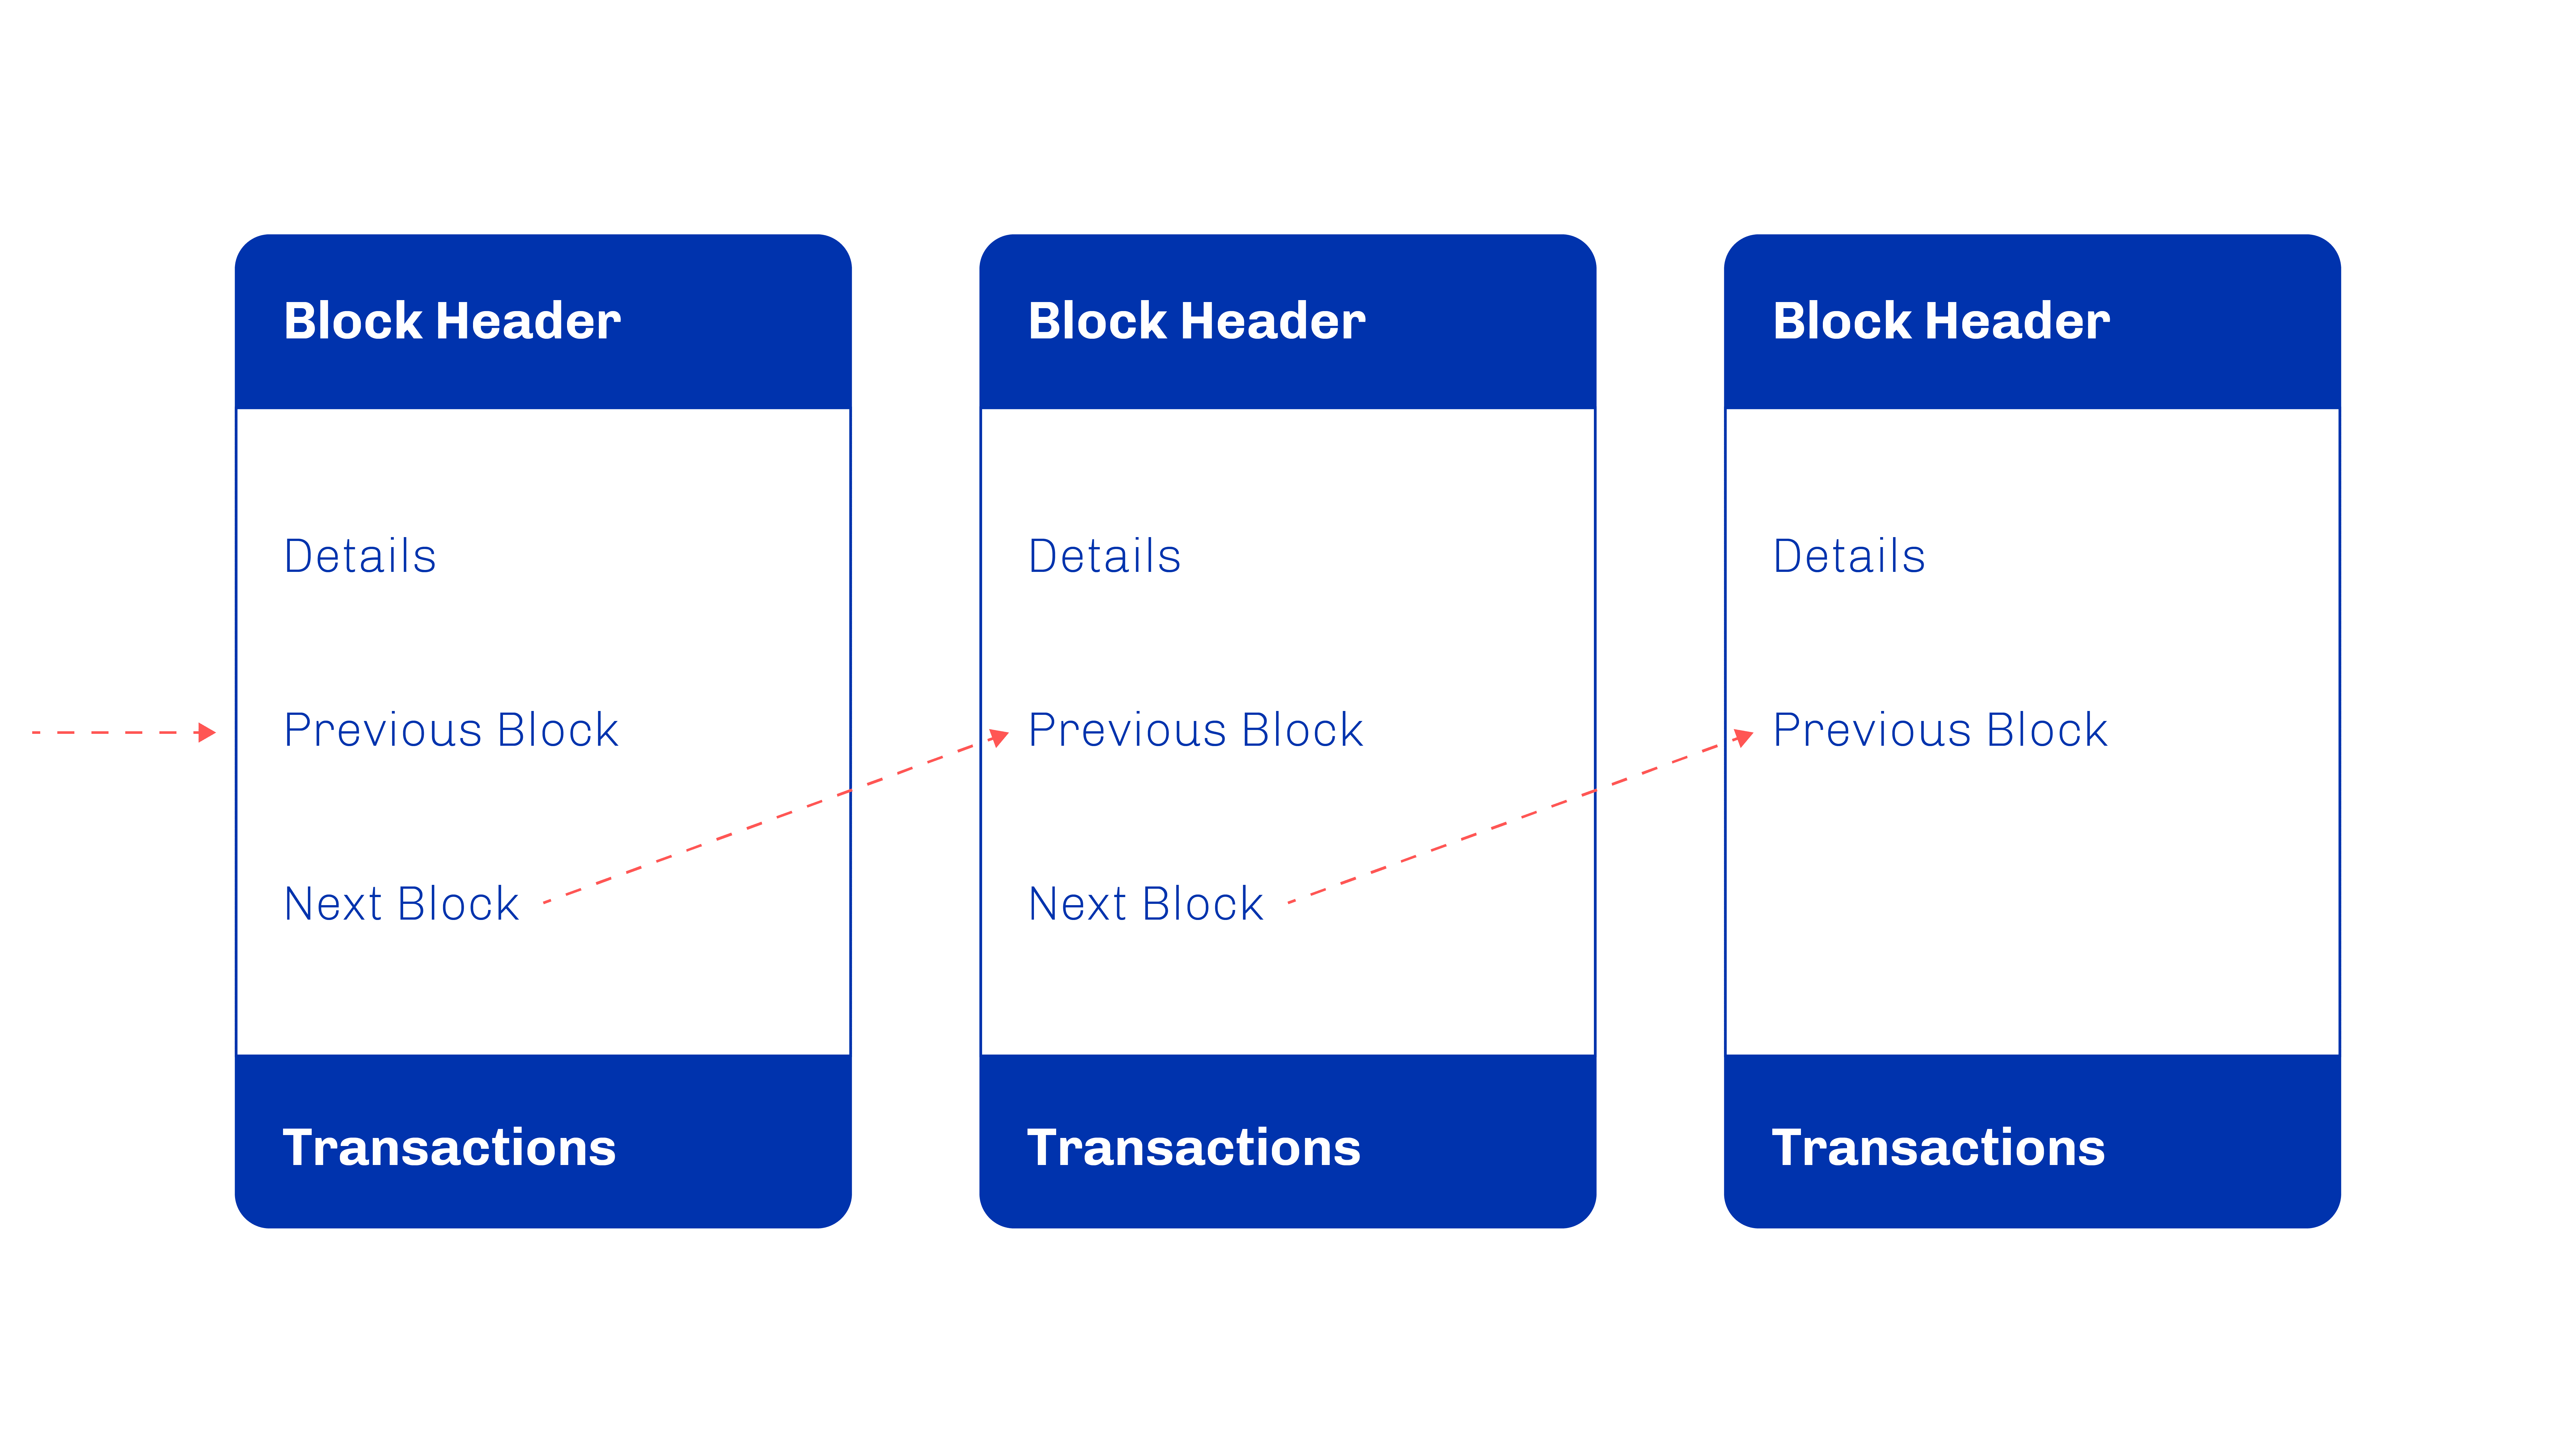
\includegraphics[width=0.9\textwidth]{Bloques.png}
	\caption{Representación simplificada de los datos en un bloque de la cadena. Extraída de~\cite{plutus-smart-contracts}.}\label{fig:Bloques}
\end{figure}

Las cadenas de bloques no solo proporcionan una base de datos inmutable y segura, sino que también actúan como un entorno funcional para realizar transacciones de fondos, crear monedas digitales y procesar transacciones complejas mediante acuerdos digitales, conocidos como \textit{smart contracts}.

% Tradicionalmente, un contrato se define como un acuerdo legalmente vinculante (por ejemplo, sobre un préstamo, venta, arrendamiento, etc). Un contrato inteligente permite forzar el cumplimiento de lo pactado en el mismo a través de una garantía asegurada por software, en la cual ninguna de las partes involucradas puede sabotear o alterar el contrato.

% De esta forma se puede renunciar a la toma de acciones legales por parte de un individuo, empresa o gobierno, y en su lugar optar por la ejecución de un programa, o contrato inteligente, para controlar la transferencia de fondos entre los participantes.
% Este objetivo se logra inmortalizando tanto el programa como su resultado en el ledger de la cadena de bloques subyacente al contrato, y garantizando así que todo el historial (incluido el estado actual del contrato) se registre de forma inmutable con un alto grado de fiabilidad. Desde la perspectiva del autor del contrato inteligente, la blockchain es un sistema de contabilidad distribuido, que realiza un seguimiento de quién posee una cantidad de un recurso virtual (Bitcoin, Ada, etc.) y cuándo los activos se transfieren de una entidad a otra.


Los propietarios de activos digitales se identifican por sus claves públicas, y pueden ser personas o máquinas.

\section{Smart contracts}

Un contrato inteligente o \textit{smart contract} es un acuerdo digital automatizado, escrito en código, que rastrea, verifica y ejecuta las transacciones vinculantes de un contrato entre varias partes. Las transacciones del contrato se ejecutan automáticamente mediante el código del smart contract cuando se cumplen las condiciones predeterminadas. Esencialmente, un contrato inteligente es un programa corto cuyas entradas y salidas son transacciones en una cadena de bloques.

Los smart contracts son auto-ejecutables y confiables y no requieren las acciones o la presencia de terceros. El código del contrato inteligente se almacena y distribuye a través de una red blockchain descentralizada, lo que lo hace transparente e irreversible.

En resumen, los contratos inteligentes son inmutables ya que no se pueden modificar, pueden distribuirse y son a prueba de manipulaciones, rápidos y rentables, ya que no hay intermediarios. Esto es seguro gracias al cifrado del mismo.

Cardano presentará el soporte de contratos inteligentes en 2021. Como un entorno funcional, Cardano apoyará el desarrollo y la implementación de contratos inteligentes utilizando lenguajes de programación como:

\begin{itemize}
	\item \textbf{Plutus}: Una plataforma de desarrollo y ejecución de smart contracts especialmente diseñada.
	      Los contratos de Plutus consisten en partes que se ejecutan en la blockchain (`código on-chain') y partes que se ejecutan en la maquina del usuario (`código off-chain o de cliente').
	      Plutus se basa en la investigación de lenguajes modernos para proporcionar un entorno de programación completo y seguro basado en Haskell, el lenguaje de programación funcional líder.

	\item \textbf{Marlowe}: Un lenguaje de dominio específico~\cite{fowler2010dsl} para escribir y ejecutar contratos financieros que permite construir contratos visualmente, así como en código más tradicional. Las instituciones financieras pueden usarlo para desarrollar e implementar instrumentos personalizados para sus clientes y usuarios. El propio lenguaje Marlowe está integrado tanto en JavaScript como en Haskell y ofrece una selección de editores según las preferencias y el conjunto de habilidades de los desarrolladores.
\end{itemize}


\section{Criptomonedas}

Las criptomonedas son activos digitales que se almacenan en el \textit{ledger} y estan diseñadas para servir como medio de intercambio de bienes o servicios. Suelen ser popularmente llamadas `criptos'.

Los ledgers de blockchain son utilizados como tecnología subyacente para la creación de criptomonedas en un entorno descentralizado. Los protocolos de blockchain utilizan técnicas criptográficas rigurosas para permitir el minting (acuñación o creación) de criptomonedas, asegurar y verificar la propiedad de las mismas y los registros de movimiento de fondos. El precio de la criptomoneda no está controlado por un gobierno o una institución financiera centralizada. Se define por su valor, la correlación con las cifras del mundo real y está impulsado por la oferta y la demanda del mercado.

Las direcciones se utilizan al enviar pagos en criptomonedas. Son identificadores únicos y están representados por una cadena de números y letras que se obtienen de las claves públicas del usuario.

\section{Cardano}

Cardano~\cite{cardano_docs} es una plataforma blockchain de tipo \textit{proof-of-stake} (prueba de participación)
\footnote{Definiciones más extensas sobre PoS se encuentran en los sitios web de \href{https://ethereum.org/en/developers/docs/consensus-mechanisms/pos/}{Ethereum} y \href{https://www.coinbase.com/es/learn/crypto-basics/what-is-proof-of-work-or-proof-of-stake}{Coinbase}}
descentralizada de tercera generación y el hogar de la criptomoneda \textit{ada}. Es la primera plataforma de cadena de bloques que evoluciona a partir de una filosofía científica y un enfoque impulsado por la investigación.

La primera generación de blockchains (con Bitcoin como gran representante) ofrecía ledgers descentralizados para la transferencia segura de criptomonedas. Sin embargo, tales cadenas de bloques no proporcionaron un entorno funcional para la liquidación de acuerdos complejos y el desarrollo de aplicaciones descentralizadas (DApps). A medida que la tecnología blockchain maduró, la segunda generación (por ejemplo Ethereum) proporcionó soluciones mejoradas para redactar y ejecutar contratos inteligentes, desarrollar aplicaciones y crear diferentes tipos de tokens. Sin embargo, la segunda generación de cadenas de bloques a menudo enfrenta problemas en términos de escalabilidad.

Cardano se concibe como la cadena de bloques de tercera generación, ya que combina las propiedades de las generaciones anteriores y evoluciona para satisfacer todas las necesidades que surjan de los usuarios. Al comparar las propiedades de las blockchains, se deben considerar muchos aspectos. Por lo tanto, la mejor solución debe garantizar la máxima seguridad, escalabilidad (rendimiento de transacciones, escala de datos, ancho de banda de la red) y funcionalidad (además del procesamiento de transacciones, la cadena de bloques debe proporcionar todos los medios para la liquidación de acuerdos comerciales). Asimismo, es importante asegurarse de que la tecnología blockchain esté en constante desarrollo en términos de sostenibilidad y sea interoperable con otras blockchains e instituciones financieras.

\begin{figure}[H]
	\centering
	
\includegraphics[width=0.5\textwidth]{Cardano_logo.png}
	\caption{Logo de la cadena de bloques Cardano. Extraído de la \href{https://en.wikipedia.org/wiki/Cardano_(blockchain_platform)}{página de Wikipedia de Cardano}.}\label{fig:Cardano_logo}
\end{figure}


La plataforma Cardano ha sido diseñada desde cero y verificada por una combinación de ingenieros y expertos académicos en los campos de blockchain y criptografía.
Tiene un fuerte enfoque en la sostenibilidad, la escalabilidad y la transparencia.
Es un proyecto totalmente de código abierto que tiene como objetivo ofrecer una infraestructura inclusiva, justa y resistente para aplicaciones financieras y sociales a escala global.

Uno de sus principales objetivos es brindar servicios financieros confiables y seguros a aquellas personas que actualmente no tienen acceso.

Cardano ha sido diseñado con la seguridad como uno de sus principios fundamentales. Está escrito en Haskell, un lenguaje de programación funcional. Los lenguajes funcionales fomentan la construcción de software usando funciones puras, lo que conduce a un diseño en el que los componentes se pueden probar convenientemente de forma aislada. Además, las funciones avanzadas de Haskell nos permiten emplear una amplia gama de métodos potentes para garantizar la corrección del código, como basar la implementación en especificaciones formales y ejecutables, pruebas exhaustivas basadas en propiedades y ejecutar pruebas en simulación.

Cardano está desarrollando una plataforma de `smart contracts' que busca ofrecer funciones más avanzadas que cualquier protocolo desarrollado anteriormente, y servirá como una plataforma estable y segura para el desarrollo de dApps de nivel empresarial.

\subsection{Ada como criptomoneda de Cardano}


Cada ledger de blockchain tiene su criptomoneda subyacente o moneda nativa. Ada es la moneda nativa o principal en Cardano. Esto significa que ada es la principal unidad de pago en Cardano; se acepta como pago de cuotas, para realizar depósitos, y también es la única moneda en la que se distribuyen las recompensas.

Lovelace es la denominación más pequeña de ada, siendo $\boxed{ 1 \text{ ada} = 1.000.000 \text{ lovelaces}}$. Ada tiene seis decimales, lo que la hace fácilmente divisible en fracciones más pequeñas.

\subsubsection{Tokens nativos}

Cardano también admite la creación de tokens nativos: activos digitales que se crean para fines específicos. Esto significa que los usuarios, desarrolladores y empresas pueden usar la cadena de bloques de Cardano para crear tokens que representen una huella de valor (ya sea definida por la comunidad, el estado del mercado o la entidad autónoma). Un token puede ser fungible (intercambiable) o no fungible\footnote{Ampliamente conocido por su acrónimo en inglés NFT} (único) y actuar como unidad de pago, recompensa, activo comercial o contenedor de información.


% Dada la importancia de los smart contracts para respaldar actividades en todos los sectores de la industria, incluyendo cadenas de abastecimiento, finanzas, servicios legales y médicos, existe una fuerte demanda de verificación y técnicas de validación sobre los mismos. Sin embargo, la gran mayoría de los contratos inteligentes carecen de cualquier tipo de especificación formal, que es esencial para establecer que el mismo es correcto.

% En este trabajo nos proponemos estudiar la verificación a bajo nivel de un grupo específico de contratos financieros definidos en el estándar ACTUS\footnote{\href{https://www.actusfrf.org/}{https://www.actusfrf.org/}}, en particular para la cadena de bloques \textit{Cardano}\footnote{\href{https://cardano.org/}{https://cardano.org/}}.

\subsection{Proof of Stake}

\textit{Proof of Stake} (PoS o Prueba de participación) es un tipo de protocolo de consenso que utiliza la cantidad de participación (o valor) mantenida en el sistema para determinar el consenso~\cite{PoS-PoW-pros-cons, PoS-PoW-energy, PoS-PoW-evaluation}.

En esencia, un protocolo de consenso es lo que controla las leyes y los parámetros que rigen el comportamiento de las cadenas de bloques. El consenso puede resumirse como un conjunto de reglas a las que se adhiere cada participante de la red.

Dado que las blockchains no están controladas por ninguna autoridad central única, en su lugar se utiliza un protocolo de consenso para permitir que los participantes del sistema distribuido acuerden el historial de la red reflejada en la cadena de bloques, para llegar a un consenso sobre lo que ha sucedido y continuar desde una sola fuente de `verdad'.

Cardano se basa en el protocolo de consenso PoS llamado Ouroboros~\cite{pof_ouroboros}, el primer protocolo de consenso de blockchain que se desarrolla a través de una investigación revisada por pares. En el corazón del protocolo se encuentran los `stake pools' (grupos de participación), nodos servidores confiables administrados por un operador de `stake pools' en los que los titulares de ada pueden delegar su participación. Los `stake pools' se utilizan para garantizar que todos puedan participar en el protocolo, independientemente de la experiencia técnica o la disponibilidad para mantener un nodo en funcionamiento.

\subsubsection{Proof of Stake vs. Proof of Work}

Por el contrario, el protocolo conocido como \textit{Proof of Work} (PoW) o prueba de trabajo es un mecanismo síncrono que anima a los mineros a competir para ser los primeros en resolver cualquier problema dentro del bloque. Se utiliza un sistema de recompensas para incentivar esta resolución de problemas. Sin embargo, este enfoque acarrea una gran desventaja, con un mayor uso de electricidad y períodos de tiempo más largos para resolver problemas dentro de la cadena. Estos factores pueden ralentizar la red significativamente y hacerla más costosa de mantener.

\subsubsection{Características del protocolo proof of stake}

Una de las características clave de PoS es que a medida que aumenta el valor del usuario, también aumenta la oportunidad de mantener el ledger; Esto significa una mayor probabilidad de producir nuevos bloques que se pueden agregar a la cadena de bloques.

El creador de un nuevo bloque se elige en función de una combinación de selección aleatoria y una medida de su participación o riqueza. Cabe aclarar que dentro de un protocolo de prueba de participación, los participantes acumulan las tarifas de transacción, lo que aumenta su riqueza a medida que avanzan. Este enfoque fomenta el crecimiento constante y estable de la blockchain y reduce los casos de transacciones estancadas que pueden impedir el crecimiento de la misma.

\subsubsection{Principales ventajas de Proof of Stake por sobre Proof of Work}

\begin{itemize}
	\item Se incorporan rigurosos protocolos de seguridad en un protocolo PoS.
	\item Centralización reducida: el riesgo de centralización se reduce al emitir sanciones por prácticas egoístas dentro de la red
	\item Eficiencia energética: el consumo de energía es extremadamente eficiente ya que se necesita una cantidad menor de electricidad, así como recursos de hardware, para producir y ejecutar la cadena de bloques.
	\item Eficiencia de costos: las monedas PoS son mucho más rentables que las que operan en los protocolos PoW.
\end{itemize}


%#########################################################################
% ESCRITURA DE CONTRATOS FINANCIEROS EN MARLOWE PARA CARDANO
%#########################################################################




\chapter[Escritura de contratos financieros en
  Marlowe]{Escritura de contratos financieros en Marlowe para Cardano}

Durante este capítulo, nos adentraremos en la escritura de contratos financieros en Marlowe. Para esto será necesario describir el modelo contable de preferencia de dichas plataformas descentralizadas, el estándar involucrado en la clasificación de los contratos financieros y el lenguaje propiamente dicho.

Al final del mismo, el lector estará familiarizado con la notación correspondiente y expondremos brevemente la especificación para un tipo de contrato.

\section{El modelo UTXO}\label{sec:UTXO} % TODO: No hay bib del libro de plutus, considero escribir la entrada por mi mismo

Para entender la estructura de los contratos en Cardano, es importante tener comprensión de como se lleva a cabo la contabilidad en la misma.
Tradicionalmente, pensamos en las transferencias de dinero entre dos cuentas bancarias, o quizás direcciones de Internet en el caso de la moneda digital.

La plataforma Cardano, asi como otras plataformas de criptomonedas como Bitcoin, utilizan en su lugar un enfoque contable conocido como UTXO~\cite{cardano_utxo_ledger} (\textit{Unspent transaction output}, o `Salidas de transacción no utilizadas').

El modelo UTXO~\cite{Translating_and_Unifying_UTXO-based, UTxO_Lars} documenta el flujo de dinero no de cuenta a cuenta, sino de \textbf{transacción a transacción}. Cada transacción tiene entradas (de dónde proviene el dinero que se gasta) y salidas (hacia donde se dirige este dinero).

Consideremos el gráfico de flujo de dinero en la figura~\ref{fig:UTXO_Funds_Flow_Example}. Las lineas negras representan outputs no gastados de las transacciones, y las lineas rojas representan dichos outputs siendo utilizados como inputs de transacciones posteriores.

Las cajas sin etiquetas representan una transacción (que contiene varios inputs y outputs). Los certificados azules denotan los outputs no gastados disponibles en nuestra ilustración.

Al comienzo del gráfico de flujo, Alice tiene 100 Ada en `outputs sin utilizar' previos al comienzo de nuestro análisis. Este dinero proviene de una o más transacciones pasadas, que exceden el alcance del gráfico. Simplificamos el mismo con una simple caja (etiquetada con su nombre y el dinero correspondiente).

Dicha caja tiene dos lineas negras (outputs) saliendo de ella, siendo la suma del valor de las mismas 100 Ada:

\begin{itemize}
	\item Un output de 58 Ada permanece sin ser utilizado y es parte de los outputs sin utilizar al final del análisis.
	\item Un output de 42 Ada se utiliza como parte de la nueva transacción.
\end{itemize}

Por su parte, Bob tiene 10 Ada de previos outputs sin utilizar. Los utiliza a todos en la nueva transacción. La transacción que ilustramos tiene dos inputs: 42 de Alice y 10 de Bob. La misma también tiene dos outputs: 2 para Bob y 50 para Charlie.

Vemos también que Charlie tiene 52 Ada provenientes de outputs previos a nuestro gráfico, totalizando 102 Ada que puede utilizar en transacciones futuras. Bob termina con solo un output de 2 Ada, y Alice con un total de 58 Ada.

\begin{figure}
	\centering
	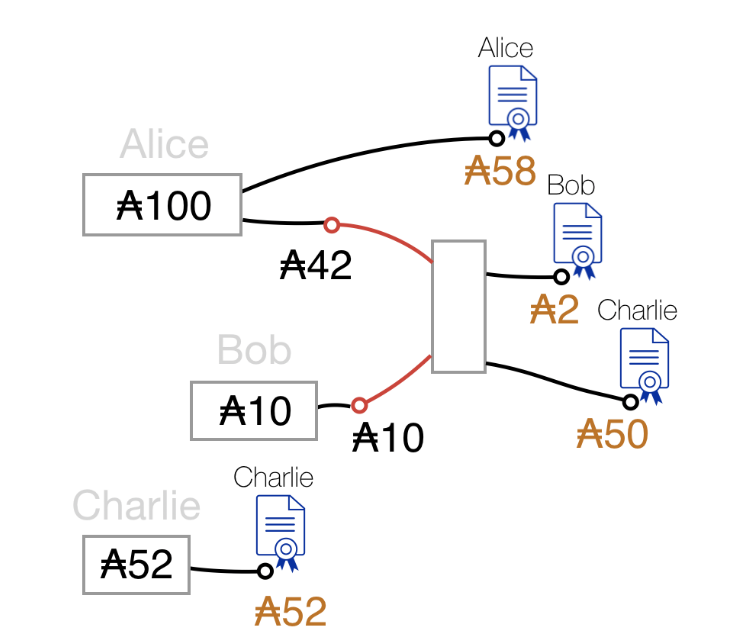
\includegraphics[width=0.7\textwidth]{UTXO_Funds_Flow_Example.png}
	\caption{Flujo de dinero en el modelo UTXO.\@ Extraído de~\cite{plutus-smart-contracts}.}\label{fig:UTXO_Funds_Flow_Example}
\end{figure}

El modelo anterior muestra estrictamente el flujo de dinero entre varios participantes. En esta versión simplificada, por ejemplo, las transacciones ilustradas no pagan comisiones. Sin embargo, en este modelo simplificado, vemos que los outputs deben gastarse en su totalidad. Es decir, un registro de un output no gastado no puede ser modificado (esta acción se adecúa a los modelos contables basados en cuentas), solo podría utilizarse de forma completa.

Para mantener la integridad de la contabilidad, las nuevas transacciones debe tener todas las outputs no gastados (totalizando la cantidad correcta de outputs no gastados) utilizados como entrada.

En nuestro ejemplo anterior, la nueva transacción elimina (utilizándolas como entrada) a los outputs no gastados de valor 42 de Alice y 10 de Bob, para un total de 52 Ada. Esto implica que la transacción esta obligada a totalizar 52 Ada como outputs sin gastar (que de hecho cumple, con 2 para Bob y 50 para Charlie).

Un aspecto a destacar es que Bob tiene un `unspent output' como entrada y uno como salida. Esto se podría interpretar como un `cambio' (de 2 Ada) para esta transacción. Dicho concepto es similar al que utilizamos en el día a día al realizar pagos en efectivo: Si un producto cuesta \$98 y tenemos un billete de \$100, no podemos fraccionar dicho billete. Tenemos que pagar con todo el billete y recibir \$2 de cambio.

Dado que no existe una forma real de gastar parte de un `unspent output', así es como el modelo UTXO trata el gasto parcial: agregando una salida de `cambio'.

Cabe destacar que este modelo contable hace que sea conveniente distribuir el flujo de efectivo de varios contribuyentes a varios destinatarios haciendo que el mismo fluya hacia un fondo común, en este caso, la transacción, antes de enviarse a los beneficiarios finales. Esto representa, en un sentido muy general, el objetivo de los `smart contracts' o contratos inteligentes.

Veamos más formalmente lo que sucede durante una transacción en el modelo UTXO.\@Para el modelo de transacciones básico que analizaremos, podemos referirnos a las siguientes definiciones:

\textbf{Datos primitivos}:

\begin{center}
	\begin{tabular}{ r @{} c @{} l r }
		txid & \ $\in$\ \  & TxId & id de transacción  \\
		ix   & \ $\in$\ \  & Ix   & índice             \\
		addr & \ $\in$\ \  & Addr & dirección          \\
		c    & \ $\in$\ \  & Coin & valor de la divisa \\
	\end{tabular}
\end{center}

\textbf{Datos derivados}:

\begin{center}
	\begin{tabular}{ r @{} c @{} l c r @{} c @{} l r}
		tx      & \ $\in$\ \  & Tx      & = & (inputs, outputs)    & \ $\in$\ \  & $\mathbb{P}(\text{TxIn}) \times$ (Ix $\mapsto$ TxOut) & transacción               \\
		txin    & \ $\in$\ \  & TxIn    & = & (txid, ix)           & \ $\in$\ \  & TxId $\times$ Ix                                      & entrada de la transacción \\
		txout   & \ $\in$\ \  & TxOut   & = & (addr, c)            & \ $\in$\ \  & Addr $\times$ Coin                                    & salida de la transacción  \\
		utxo    & \ $\in$\ \  & UTxO    & = & txin $\mapsto$ txout & \ $\in$\ \  & TxIn $\mapsto$ TxOut                                  & salidas sin gastar        \\
        b       & \ $\in$\ \  & Block   & = & \{tx\}                   & \ $\in$\ \  & $\mathbb{P}(\text{Tx})$                               & bloque                    \\
        pending & \ $\in$\ \  & Pending & = & \{tx\}                   & \ $\in$\ \  & $\mathbb{P}(\text{Tx})$                               & transacciones pendientes
	\end{tabular}
\end{center}

\textbf{Funciones:}

\begin{center}
	\begin{tabular}{ r @{} c @{} l r }
		txid & \ $\in$\ \  & Tx $\mapsto$ TxId       & computar id de la transacción               \\
		ours & \ $\in$\ \  & Addr $\mapsto \mathbb{B}$ & direcciones que corresponden a la billetera \\
	\end{tabular}
\end{center}

\textbf{Filtros sobre Conjuntos}:

\begin{center}
	\begin{tabular}{ r @{} c @{} l}
		$\text{Addr}_{ours}$  & \ =\ \  & $\{a\ |\ a \in \text{Addr},\ \text{ours}\ a\}$ \\
		$\text{TxOut}_{ours}$ & \ =\ \  & $\text{Addr}_{ours}$ $\times$ Coin             \\
	\end{tabular}
\end{center}

% \begin{figure}[H]
%     \centering
%     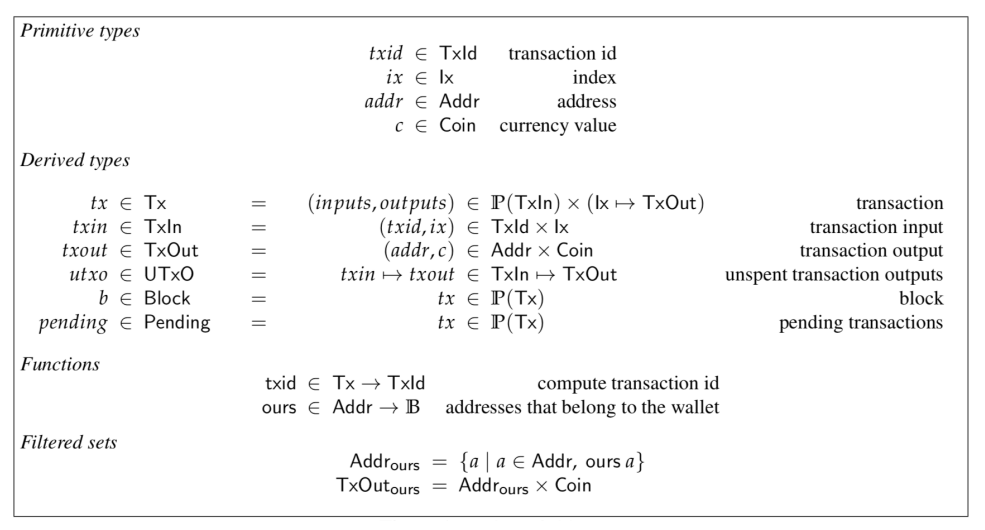
\includegraphics[width=0.9\textwidth]{Basic_UTXO_Definitions.png}
%     \caption{Definiciones básicas en el modelo UTXO.\@ Extraído del libro `\textit{Plutus: Writing reliable smart contracts}'}\label{fig:Basic_UTXO_definitions}
% \end{figure}

Antes de analizar la estructura de las transacciones, haremos un pequeño repaso sobre como la contabilidad se lleva a cabo en el `libro mayor' o ledger. El registro que contiene la información sobre el ledger es llamado \texttt{UTXO}. Este registro es un map finito, donde la key o clave is un par formado por el id de la transacción de la cual se toma el dinero y un indice, \texttt{TxIn = TxId * Ix}. El id de la transacción puede ser calculado en base a una transacción completada para procesar, y es un identificador único de la transacción.

El índice \texttt{Ix} es necesario debido a que puede haber mas de un output en dicha transacción, y cada uno de los mismos tiene que tener un identificador único dentro de el conjunto de `outputs' dentro de una transacción.

Los valores o `values' en el mapa son pares formados por un `coin value' y una dirección, y el tipo de los mismos es \texttt{TxOut = Addr * Coin}. Cabe destacar que las direcciones de los usuarios son siempre claves públicas, y los fondos en ellas pertenecen a la entidad que puede probar que posee la clave privada correspondiente. Las direcciones de `script' (smart contract o contrato inteligente) se comportan de manera ligeramente distinta, debido a que no tienen un dueño directo.

Para poder comprender la estructura de la transacción en sí, analicemos primero los `outputs'. Una transacción puede distribuir el dinero que está gastando a varias direcciones diferentes. Los outputs, (valores de tipo \texttt{TxOut}) se almacenan en una transacción como valores en un mapa finito.
Las claves del mapa son indices únicos dentro del contexto del mapa, de manera tal que la combinación del id de la transacción y dicho indice identifica de forma global a dicho output.
En el modelo UTXO, se relaciona a los valores de salida con las entradas de las cuales provienen, por medio de este identificador global compuesto.


Los inputs, cuyo orden no es relevante, son un conjunto y no una lista. Los elementos de este conjunto no contienen ni el valor de la moneda a gastar, ni la dirección de donde proviene el dinero. Esta es la principal distinción entre el modelo contable tradicional y el UTXO:\@el dinero que se gasta solo referencia a los outputs no gastadas de transacciones previamente procesadas en el `ledger' que reside actualmente en la blockchain. Cada elemento del mencionado set de inputs es un par formado por el id de la transacción y un indice que, como se explicó anteriormente, identifica de forma única el output no gastado en la UTXO.\@

Procesar una transacción implica actualizar el \texttt{UTXO} en el ledger de manera tal que los fondos gastados por la transacción que se está procesando estén disponibles para que los gasten los propietarios de las direcciones de las salidas de la transacción. Es decir, todas las entradas correspondientes a inputs de la transacción procesada se eliminan del ledger \texttt{UTXO}.

Adicionalmente, todos los valores de \texttt{TxOut} en el mapa finito de las salidas de la transacción se agregan a la \texttt{UTXO}, con la clave del mapa finito que consiste en el id de la transacción que se procesa, y el valor del índice es el mismo que en el mapa finito de salidas de esta transacción. Es decir, si \texttt{tx} contiene un par formado por el conjunto de entrada y el mapa de salidas \texttt{(ins, outs)} con id \texttt{id}, y \texttt{ix |-> (a, c)} es una entrada de \texttt{outs}, la \texttt{UTXO} va a tener la entrada \texttt{(id, ix) |-> (a, c)} agregada. En este párrafo, utilizamos la notación \texttt{k |-> v} para referirnos a una entrada del mapa finito con clave \texttt{k} y valor \texttt{v}.

Veamos como se refleja dicha actualización del ledger en términos de notación matemática (que puede ser reflejada en código con relativa facilidad). Las siguientes son tres formas de filtrar el mapa finito de \texttt{UTXO}. El primero filtra dicho mapa mediante un subconjunto \texttt{ins} de las claves. El segundo filtro obtiene el complemento del resultado del primer filtro (en otras palabras, todas las entradas de la \texttt{UTXO} que no son indexadas por claves en la lista de inputs). El tercero filtra el mapa mediante los valores.

\begin{center}
	\begin{tabular}{ r @{} c @{} l r }
		\texttt{ins} $\lhd$ \texttt{utxo}           & \ =\ \  & $\{ i \mapsto o\ |\ i \mapsto o \in utxo,\ i \in ins \}$    & restricción de dominio \\
		\texttt{ins} $\ntriangleleft$ \texttt{utxo} & \ =\ \  & $\{ i \mapsto o\ |\ i \mapsto o \in utxo,\ i \notin ins \}$ & exclusión de dominio   \\
		\texttt{utxo} $\rhd$ \texttt{outs}          & \ =\ \  & $\{ i \mapsto o\ |\ i \mapsto o \in utxo,\ o \in outs \}$   & restricción de rango
	\end{tabular}
\end{center}

Utilizaremos la notación introducida para procesar una nueva transacción. En otras palabras, eliminar los outputs no gastados correspondientes y construir un nuevo conjunto de outputs que serán agregados al \texttt{UTXO} (como se describió anteriormente). Los outputs a agregar serían computados de la siguiente manera:

\begin{center}
	\begin{tabular}{|r c l|}
		\hline               &       &                                                             \\
		$\text{txins}$       & $\in$ & $\mathbb{P}(\text{Tx}) \rightarrow \mathbb{P}(\text{TxIn})$ \\&&\\

		$\text{txins } txs$  & =     & $\bigcup \{ inputs\ |\ (inputs, \_ ) \in txs$\}             \\&&\\

		$\text{txouts}$      & $\in$ & $\mathbb{P}(\text{Tx}) \rightarrow \text{UTXO}$             \\&&\\

		$\text{txouts } txs$ & =     &
		$\left \{
			\begin{array}{l|lcl}
				                                    & tx               & \in & txs     \\
				(\text{txid } tx, ix) \mapsto txout & (\_, outputs)    & =   & tx      \\
				                                    & ix \mapsto txout & \in & outputs \\
			\end{array}
		\right \} $                                                                                 \\&&\\
		\hline
	\end{tabular}
\end{center}

Usando esta notación, podemos definir la actualización del \texttt{UTXO}, debido a la transacción \texttt{tx} como:

\[ (\text{txins } tx\ntriangleleft\ utxo) \cup\text{outs } tx \]

Hay que tener en cuenta que se debe realizar un cálculo explícito de la cantidad total de Aca en las salidas y el total de \textit{ada} en todas las entradas de una transacción como parte de la validación de la transacción. También podría haber outputs en una transacción sin inputs correspondientes; estos se deben a la recolección de recompensas.

Ahora, para validar una transacción, se realiza una serie de cálculos que involucran el Ada en la misma y el Ada en otras cuentas del ledger, para asegurarse de que no se crea ni se destruye dinero. Esto se conoce como `propiedad contable generalizada'. El modelo contable UTXO brinda protección integrada contra el `doble gasto' de un output determinado.

Esta protección inherente, junto con la aplicación de la propiedad contable generalizada, asegura que no se permita que ocurra ningún gasto deshonesto. Esta es una propiedad crucial del sistema contable del ledger de Cardano, en particular porque existe una cantidad fija de Ada que nunca puede cambiar.

Para finalizar, hay que tener en cuenta que una transacción incluye una gran cantidad de datos adicionales, como testigos, certificados, y scripts juntos con sus hashes. En esta sección no hemos entrado en los detalles de los tipos y cálculos específicos utilizados en la implementación del ledger de Cardano. Sin embargo, abarcamos suficiente información como para poder entender que sucede detrás de escena cuando se genera una transacción en la blockchain.


\section{Marlowe como DSL}
Marlowe~\cite{implementing_financial_contracts_on_blockchain, standardized_crypto_loans} es un lenguaje pequeño, con pocas sentencias soportadas que, para cada contrato, describen el comportamiento que involucra un conjunto fijo y finito de roles.

Marlowe está diseñado para crear bloques para contratos financieros: pagos o depósitos de las partes, elecciones e información del mundo real. Cuando se ejecuta un contrato, los roles que implica son satisfechos por los participantes, que son identidades en la cadena de bloques. Cada rol está representado por un token en la cadena y los roles se pueden transferir durante la ejecución del contrato, lo que significa que esencialmente se pueden intercambiar.

Los contratos se pueden construir reuniendo una pequeña cantidad de estas sentencias que, en combinación, se pueden usar para describir y modelar muchos tipos diferentes de contratos financieros. Algunos ejemplos incluyen un contrato que puede realizar un pago a un rol o a una clave pública, un contrato que puede esperar una acción por parte de uno de los roles, como un depósito de moneda, o una elección entre un conjunto de opciones.

En particular, un contrato no puede esperar indefinidamente una acción: si la misma no se ha realizado en un tiempo determinado (conocido como \textit{timeout}), el mismo continuará con un comportamiento alternativo, por ejemplo, reembolsar los fondos en el contrato.

Los contratos de Marlowe pueden ramificarse en función de alternativas y tienen una vida finita, al final de la cual el dinero restante retenido por el mismo se devuelve a los participantes. Esta característica garantiza que el dinero no se puede bloquear para siempre en un contrato. Dependiendo del estado actual de un contrato, se puede elegir entre dos cursos de acción alternativos, que son en sí mismos contratos. Cuando no se requieran más acciones, el contrato se cerrará y se reembolsará cualquier moneda restante en el contrato.

\subsection{El modelo de Marlowe}

Marlowe está diseñado para soportar la ejecución de contratos financieros en la blockchain, específicamente en Cardano. Los contratos se construyen reuniendo una pequeña cantidad de constructores que se pueden combinar para describir muchos tipos diferentes de contratos financieros.

Antes de describir estos constructores en~\ref{sec:constructores_marlowe}, debemos analizar el enfoque general para modelar contratos en Marlowe, y el contexto en el que se ejecutan los mismos (la blockchain de Cardano). Al hacer esto, también presentamos parte de la terminología que usaremos, indicando las definiciones en cursiva.

\subsubsection{Contratos}
Los contratos en Marlowe se ejecutan en una blockchain, pero deben interactuar con el mundo fuera de la misma. Las partes (\textit{parties}) del contrato, a las que también llamamos participantes, pueden realizar diversas acciones: se les puede pedir que depositen dinero o que elijan entre varias alternativas. Una notificación de un valor externo (también llamado valor de oráculo), como el precio actual de un producto en particular, es la otra forma posible de entrada.\footnote{Podemos pensar a los oráculos como otro tipo de \textit{party} del contrato; bajo este punto de vista, las notificaciones se convierten en las elecciones (\textit{choices}) realizadas por esa \textit{party}.}

La ejecución de un contrato también producirá efectos externos, al realizar pagos a las partes en el mismo.

\subsubsection{Participantes y roles}
Los \textit{participantes} y los \textit{roles} se comportan de forma ligeramente distinta en un contrato en Marlowe. Los roles en un contrato son fijos e inmutables, y pueden ser llamados \texttt{party}, \texttt{counterparty}, etc. Por otro lado, los participantes que están vinculados a los roles del contrato pueden cambiar durante la ejecución de la instancia de contrato en particular. Esto permite que los roles en la ejecución de contratos se intercambien entre los participantes, a través de un mecanismo de \textit{tokenización}. A la fecha de escritura de este documento, la simulación en \textit{Marlowe Playground}~\cite{marlowe_playground} simplemente presenta roles de contrato.

\subsubsection{Cuentas}
El modelo de Marlowe permite que un contrato pueda almacenar activos. Todas las partes que participan en el contrato poseen implícitamente una cuenta con su nombre. Todos los bienes almacenados en el contrato deben estar en la cuenta de una de las partes; de esta forma, cuando se cierra el contrato, todos los bienes que quedan en el contrato pertenecen a alguien, por lo que pueden ser reembolsados a sus respectivos dueños. Estas cuentas son \textit{locales}: solo existen mientras dura la ejecución del contrato, y durante ese tiempo son accesibles (solo desde dentro del contrato).

\subsubsection{Pasos y estados}
Los contratos de Marlowe describen una serie de \textit{pasos}, generalmente describiendo el primer paso, junto con otro subcontrato que describe qué hacer a continuación. Por ejemplo, el contrato \texttt{Pay a p t v cont} dice ``realice un pago del valor \texttt{v} del token \texttt{t} a la parte \texttt{p} desde la cuenta \texttt{a}, y luego siga el contrato \texttt{cont}''. Llamamos \texttt{cont} a la continuación del contrato.

Al ejecutar un contrato, debemos realizar un seguimiento del \textit{contrato actual}: después de dar un paso en el ejemplo anterior, el contrato actual es la continuación, \texttt{cont}. También tenemos que realizar un seguimiento de información adicional, como por ejemplo: cuánto se tiene en cada cuenta. Llamamos a esta información el \textit{estado}: este también cambia potencialmente en cada paso. Un paso también puede implicar que se lleva a cabo una acción, como el depósito de dinero o la producción de un \textit{efecto}, por ejemplo un pago.

\subsubsection{Blockchain}

Si bien Marlowe está diseñado para trabajar con cadenas de bloques en general, algunos detalles de cómo interactúa con la misma son relevantes al describir la semántica y la implementación del lenguaje.

Una cadena de bloques basada en UTXO~\ref{sec:UTXO} contiene una coleccion de transacciones. Cada transacción tiene un conjunto de entradas y salidas, y la cadena de bloques se construye vinculando las salidas de transacciones no gastadas (UTXO) a las entradas de una nueva transacción. Como máximo se puede generar un bloque en cada \textit{slot}, que tienen una duración de 1 segundo.

Los mecanismos por los cuales se generan estos bloques, y por quién, no son relevantes para el alcance de este documento, pero los contratos se expresarán en términos de números de \textit{slot}, contados desde el bloque de inicio (``génesis'') de la cadena de bloques. Actualmente, utilizan números de \textit{slot} en la simulación en el Marlowe Playground~\cite{marlowe_playground}, pero en cadena usaremos el tiempo, adoptando el estándar de tiempo Posix.

\subsubsection{UTXO, billeteras y la aplicación Marlowe Run}
El dinero dentro de la blockchain reside en los UTXO, que están protegidos criptográficamente por una clave privada en poder del propietario. Estas claves se pueden usar para canjear la salida y usarlas como entradas para nuevas transacciones. Los usuarios suelen realizar un seguimiento de sus claves privadas y los valores adjuntos a ellas en una billetera (o \textit{wallet}) criptográficamente segura.

Para interactuar con un contrato que se ejecuta en blockchain, los usuarios deberán usar la aplicación cliente \textit{Marlowe Run}. Esta interactuará con las billeteras de los usuarios para autenticar las transacciones que gastan criptoactivos, ya que los depósitos se realizan desde las billeteras de los usuarios y los pagos son recibidos por ellos. El código que realiza este tipo de acciones suele ser llamado \textit{off-chain}, debido a que no queda inmortalizado en la misma.

\subsubsection{Simulación omnisciente}
El Playground de Marlowe~\cite{marlowe_playground} admite la simulación de contratos. Esta es una simulación omnisciente, en la que el usuario puede realizar cualquier acción para cualquier rol y, por lo tanto, puede observar la ejecución desde la perspectiva de todos los usuarios simultáneamente. Esto contrasta con la experiencia de ejecutar un contrato en Marlowe Run, en el que cada participante ve el contrato desde su propio punto de vista. En particular, los participantes solo pueden interactuar con un contrato en ejecución que está esperando su entrada; si ese no es el caso, entonces verán que la ejecución del contrato está esperando la participación de otra persona.

\subsubsection{Valores y \textit{tokens}}
En los ejemplos de los capítulos posteriores, veremos que siempre que se requiere un \textit{valor}, hemos utilizado exclusivamente \textit{Ada}. Esto tiene sentido ya que \textit{Ada} es la moneda fundamental respaldada por Cardano.

Sin embargo, Marlowe ofrece un concepto de \textit{valor} más general, que admite tokens \textit{nativos} personalizados, que pueden ser fungibles, no fungibles o mixtos:

\begin{lstlisting}[style=Haskell-cardano, caption=Definicion del tipo \texttt{Value}]
newtype Value = Value
    {getValue :: Map CurrencySymbol (Map TokenName Integer)}
\end{lstlisting}

Los tipos \texttt{CurrencySymbol} y \texttt{TokenName} son wrappers simples alrededor de \texttt{ByteString}.


Esta noción de valor abarca a \textit{Ada}, tokens fungibles (como monedas), tokens no fungibles o NFT (tokens personalizados que no son intercambiables con otros tokens) y casos mixtos más exóticos:

\begin{itemize}
    \item Ada usa la cadena de bytes vacía como \texttt{CurrencySymbol} y \texttt{TokenName}.

    \item Un \textit{token fungible} está representado por un \texttt{CurrencySymbol} (o símbolo de moneda) para el que existe exactamente un \texttt{TokenName} (nombre de token) que puede tener una cantidad entera arbitraria no negativa (del cual \textit{Ada} es un caso especial).

    \item Una clase de \textit{tokens no fungibles} es un \texttt{CurrencySymbol} con varios \texttt{TokenName}s, cada uno de los cuales tiene una cantidad de uno. Cada uno de estos nombres corresponde a un \textit{token único no fungible}.

    \item Los \textit{tokens mixtos} son aquellos que tienen varios \texttt{TokenName}s y cantidades superiores a uno.

\end{itemize}

\subsubsection{Ejecución de un contrato Marlowe}
Ejecutar un contrato de Marlowe en la cadena de bloques de Cardano significa restringir las transacciones generadas por el usuario a la lógica del contrato. Si en un punto particular de ejecución, un contrato espera un depósito de \texttt{100 Ada} de Alice, solo esa transacción tendrá éxito, cualquier otra será rechazada.

Una transacción contiene una lista ordenada de \textit{entradas} o \textit{acciones}. El intérprete de Marlowe se ejecuta durante la validación de transacciones. Primero, evalúa el contrato \textit{paso} a \textit{paso} hasta que no se puede cambiar más sin procesar ninguna entrada, una condición que se llama \textit{quiescent} (o inactiva). En esta etapa, avanza a través cualquier \texttt{When} con tiempos de espera que hayan pasado, y todos los constructores \texttt{If}, \texttt{Let}, \texttt{Pay} y \texttt{Close}, sin procesar ninguna entrada.

A continuación, se procesa la primera entrada, y luego el contrato se vuelve a procesar hasta la inactividad. Este proceso se repite hasta que se procesan todas las entradas. En cada paso, el contacto actual y el estado cambiarán, es posible que se procesen algunas entradas y se realicen pagos.

Tal \textit{transacción}, como se muestra en el diagrama a continuación, se agrega a la cadena de bloques. 

Hemos mostrado que el comportamiento de un Marlowe es independiente de cómo se recopilan las entradas en las transacciones, por lo que cuando simulamos la acción de un contrato no necesitamos agrupar las entradas en transacciones explícitamente. Para ser más concretos, podemos pensar que cada transacción tiene como máximo una entrada. Si bien la semántica de un contrato es independiente de cómo se agrupan las entradas en transacciones, los costos de ejecución pueden ser menores si se pueden agrupar varias entradas en una sola transacción.

En la simulación omnisciente disponible en el \textit{Playground}, podemos abstraernos con seguridad de la agrupación de transacciones, ya que la agrupación no afecta el comportamiento del contrato.

\subsubsection{Construyendo una transacción}

\begin{figure}[H]
    \centering
    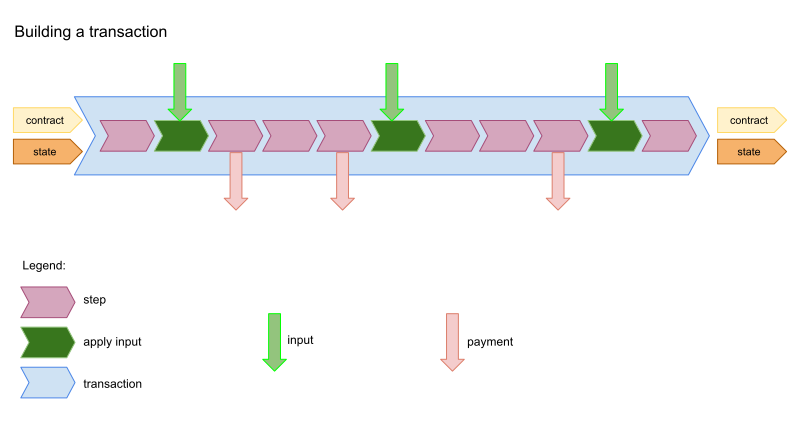
\includegraphics[width=0.8\textwidth]{Transaccion.png}
    \caption{Diagrama de ejemplo de una transacción. Extraído de \href{https://play.marlowe-finance.io/doc/marlowe/tutorials/marlowe-model.html}{https://play.marlowe-finance.io/doc/marlowe/tutorials/marlowe-model.html}.}\label{fig:Transaccion}
\end{figure}


\subsection{Piezas fundamentales de un contrato en Marlowe}\label{sec:constructores_marlowe}
Un contrato en Marlowe se obtiene combinando una pequeña cantidad de sentencias o \textit{building blocks}. Las mismas pueden llegar a describir muchos tipos de contratos financieros, como hacer un pago, hacer una observación, esperar hasta que cierta condición se cumpla, etc. Luego, el contrato se ejecuta en una cadena de bloques, como Cardano, e interactúa con el mundo exterior.

Marlowe en sí mismo está embebido en Haskell, y se modela como una colección de tipos de datos algebraicos en Haskell~\cite{Algebraic_data_type}. A continuación mostramos la definición más general de un contrato en Marlowe:

\begin{lstlisting}[style=Haskell-cardano, language=Marlowe, caption=Tipos de contratos en Marlowe.]
data Contract = Close
              | Pay party payee token value contract
              | If observation contract1 contract2
              | When [Case] timeout contract
              | Let valueId value contract
              | Assert observation contract
\end{lstlisting}

Marlowe tiene seis maneras de construir contratos. Cinco de esos métodos ---
\texttt{Pay}, \texttt{Let}, \texttt{If}, \texttt{When}, y \texttt{Assert} --- construyen un contrato complejo a partir de contratos más simples, y el ultimo método, \texttt{Close} es un contrato simple. En cada paso de la ejecución, además de modificar el estado y proceder hacia un nuevo contrato, podrían generarse pagos y advertencias (\textit{warnings}).

Antes de describir los métodos exhaustivamente, es útil conocer la definición de valores, observaciones y acciones:

\begin{enumerate}
    \item \textbf{Valores (\textit{values})}: Incluyen cantidades que cambian con el tiempo, tales como: el \textit{slot interval} o `intervalo actual', el balance de cierto token en una cuenta o elecciones que se han realizado (conocidas como \textit{valores volátiles}). Los valores pueden ser combinados usando operaciones como suma, resta, negación, etc. Los mismos pueden ser valores condicionales o una observación.

	\item \textbf{Observaciones (\textit{observations})}: Valores booleanos que son obtenidos al comparar valores, y que pueden ser combinados con los operadores booleanos estándar. Además, es posible observar si alguna elección se ha realizado (para una elección en concreto). Las observaciones tendrán un valor en cada etapa de la ejecución.

	\item \textbf{Acciones (\textit{actions})}: Suceden en momentos particulares durante la ejecución, por ejemplo: un depósito de dinero o elegir entre varias alternativas.
	      % Revisar oracles, que parecen haber sido incluidos, pero no estoy seguro de si son relevantes o no para nuestro trabajo.
\end{enumerate}


\subsubsection{Pay}
Un contrato de pago \texttt{(Pay acc payee tok val cont)} realizará un pago de valor \texttt{val} de un token \texttt{tok} desde una cuenta \texttt{acc} a un beneficiario \texttt{payee}, quien sera uno de los participantes del contrato, u otra cuenta en el mismo.

Se generarán \textit{warnings} si el valor \texttt{val} no es positivo, o si no hay recursos suficientes en \texttt{acc} para realizar el pago en su totalidad (incluso si hay balances positivos de otros tokens en la misma). En este último caso, se realizará un pago parcial (conteniendo todo el dinero disponible). El contrato en el que continuará la ejecución es \texttt{cont}.

\subsubsection{Close}\label{sec:Close}

Un contrato \texttt{Close} prevé que el contrato sea cerrado (o rescindido). La única acción que realiza es reembolsar a los titulares de cuentas que contienen un saldo positivo. Esto se realiza de a una cuenta a la vez, pero todas las cuentas se reembolsarán en una sola transacción.

\subsubsection{If}
El conditional \texttt{If obs cont1 cont2} continuará en \texttt{cont1} o \texttt{cont2}, dependiendo de la observación \texttt{obs} cuando el mismo es ejecutado.

\subsubsection{When}
Es el constructor de contratos mas complejo, con la forma \texttt{When cases timeout cont}. El mismo es activado por acciones, que pueden o no ocurrir en un \textit{slot} en particular. Como continua el mismo tras una acción se declara en la sintaxis de \texttt{cases} del contrato.

En el contrato \texttt{When cases timeout cont}, la lista \texttt{cases} contiene una colección de casos. Cada caso es de la forma \texttt{Case ac co} donde \texttt{ac} es una acción y \texttt{co} un contrato de continuación. Cuando una acción en particular, por ejemplo \texttt{ac}, ocurre, el estado del contrato es actualizado correspondientemente y y mismo continuara su ejecución en \texttt{co}.

Para garantizar que el contrato eventualmente progresará, la ejecución de \texttt{When cases timeout cont} continuará como \texttt{cont} una vez que el slot \texttt{timeout} es alcanzado.

\subsubsection{Let}

Un contrato \texttt{Let id val cont} permite registrar un valor, en un punto particular en el tiempo, y darle nombre usando un identificador. En este caso, la expresión \texttt{val} se evalúa y se almacena con el nombre \texttt{id}. El contrato entonces continúa como \texttt{cont}.

Además de permitirnos usar abreviaturas, este mecanismo nos brinda la capacidad de capturar y guardar valores volátiles que pueden cambiar con el tiempo, por ejemplo: '\textit{el precio actual del petróleo}', '\textit{el slot actual, en un punto particular de la ejecución del contrato}', para ser utilizado más adelante en la ejecución del mismo.

\subsubsection{Assert}
Un contrato \texttt{Assert obs cont} no tiene ningún efecto en el estado de un contrato, que continua inmediatamente en \texttt{cont}, pero genera una advertencia cuando la observación \texttt{obs} es falsa. Puede ser utilizado para asegurar que alguna propiedad se cumple en un momento particular de la ejecución del contrato. Esta sentencia es útil porque permite que un \textit{análisis estático} detecte que algún \texttt{assert} es falso, para alguna ejecución específica del contrato.


\section{Un contrato de ejemplo en Marlowe}

Esta sección introduce un contrato financiero simple en pseudocódigo y luego explicá como puede ser modificado para funcionar en Marlowe, dando el primer ejemplo de un contrato en el lenguaje. La misma se basa principalmente en el contrato de ejemplo brindado por la documentación oficial\footnote{Disponible en \href{https://play.marlowe-finance.io/doc/marlowe/tutorials/escrow-ex.html}{https://play.marlowe-finance.io/doc/marlowe/tutorials/escrow-ex.html}}.

\subsection{El contrato \textit{Escrow}}

Supongamos que Alice quiere comprarle un libro a Bob, pero ninguno de los dos confía en el otro. Afortunadamente, tienen una amiga en común, Carol, en quien ambos confían para que sea neutral (pero no lo suficiente como para darle el dinero y actuar como intermediaria). Entonces, acuerdan el siguiente contrato, escrito en pseudocódigo funcional. Este tipo de contrato es un ejemplo simple de depósito en garantía o \textit{escrow}:


\begin{lstlisting}[style=Haskell-cardano, language=Marlowe, caption=Primer pseudocódigo del contrato Escrow.]
When aliceChoice
     (When bobChoice
           (If (aliceChosen `ValueEQ` $\backtick$ bobChosen)
               agreement
               arbitrate))
\end{lstlisting}


El contrato se describe utilizando los constructores vistos en la sección previa. El constructor más externo \texttt{When} tiene dos argumentos: el primero es una observación y el segundo es otro contrato. El significado esperado es que cuando ocurre la acción, se activa el segundo contrato.

El segundo contrato es en sí mismo otro \texttt{When} --- esperando una decisión de Bob --- pero dentro de este, hay una opción: Si (\texttt{If}) Alice y Bob están de acuerdo en qué hacer, se procede; en caso contratio, se le pide a Carol que arbitre y tome una decisión.

En general, \texttt{When} ofrece una lista de casos\footnote{Las listas en Marlowe se representan entre corchetes, como en \texttt{[2,3,4]}.}, cada uno con una acción y un contrato correspondiente que se activa cuando ocurre esa acción. Sabiendo esto, podemos permitir la opción de que Bob realice la primera elección, en lugar de Alice, de la siguiente forma:

\begin{lstlisting}[style=Haskell-cardano, language=Marlowe, caption=Pseudocódigo agnóstico al orden de las elecciones.]
When [ Case aliceChoice
            (When [ Case bobChoice
                        (If (aliceChosen `ValueEQ` bobChosen)
                           agreement
                           arbitrate) ],
      Case bobChoice
            (When [ Case aliceChoice
                        (If (aliceChosen `ValueEQ` bobChosen)
                            agreement
                            arbitrate) ]
     ]
\end{lstlisting}

En este contrato, Alice o Bob pueden hacer la primera elección y el otro luego hará la siguiente. Si están de acuerdo, entonces se procede con el mismo; en caso contrario, Carol arbitra. En esta sección, y sin perdida de generalidad, supondremos que Alice elige primero (esto nos permite omitir el codigo simétrico y repetido que cubriría el caso en el que Bob comienza).

A coninuación, se incluye un diagrama de secuencia que ilustra el comportamiento esperado del contrato, descripto anteriormente en pseudocódigo:

\begin{figure}[H]
    \centering
    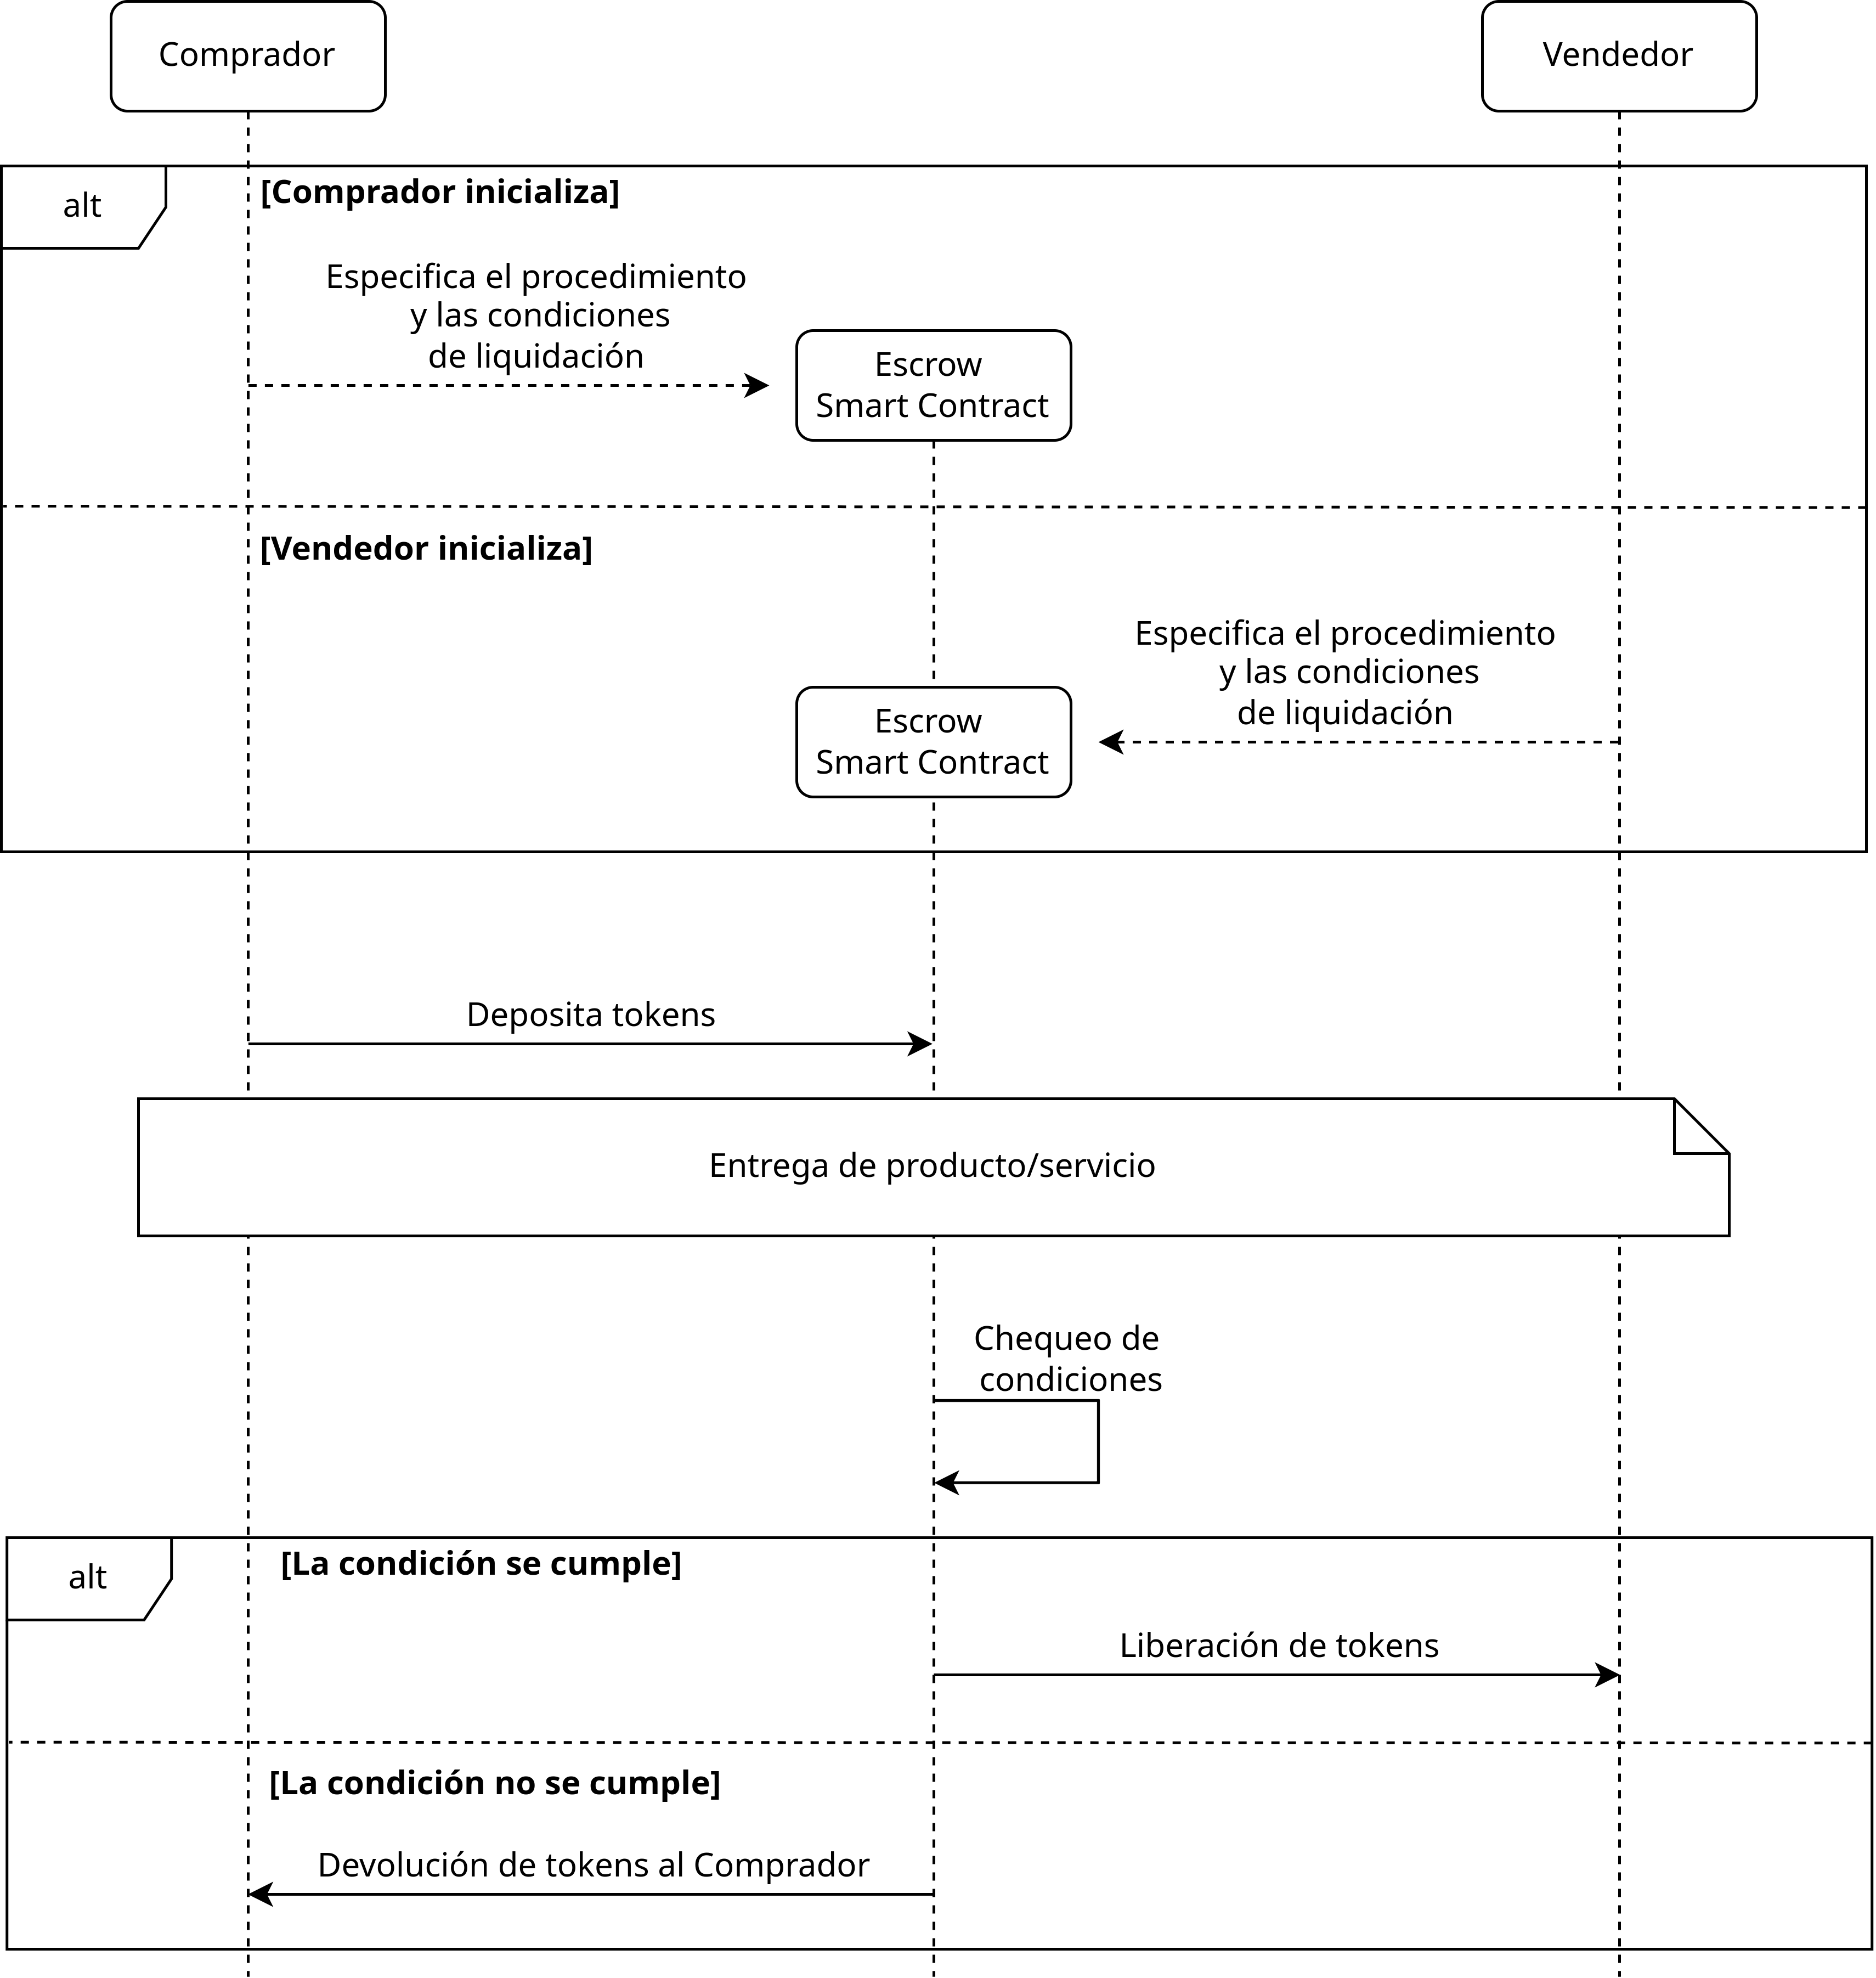
\includegraphics[width=\textwidth]{Escrow.png}
    \caption{Diagrama de secuencia del contrato \textit{Escrow}.}\label{fig:Escrow}
\end{figure}

En~\cite{composing-contracts, multi-party-contracts} se encuentran los trabajos iniciales sobre la utilización de programación funcional para la descripción de contratos financieros.

\subsection{Escrow en Marlowe}

Los contratos de Marlowe incorporan parametros adicionales para garantizar que progresen correctamente. Cada vez que vemos un \texttt{When}, debemos proporcionar dos cosas adicionales:

\begin{itemize}
    \item El tiempo de espera (o \textit{timeout}) luego del cual el contrato progresará.
    \item El contrato de continuación al que progresa.
\end{itemize}

\subsubsection{Agregando \textit{timeouts}}

Primero, examinemos cómo modificar el pseudocódigo escrito para solucionar el caso de que la condición del \texttt{When} no se cumpla. Para eso, agregamos valores de \textit{tiemout} y `contrato de continuación' para cada \texttt{When} en el contrato:

\begin{lstlisting}[style=Haskell-cardano, language=Marlowe, caption=Pseudocódigo con timeouts.]
When [ Case aliceChoice
            (When [ Case bobChoice
                        (If (aliceChosen `ValueEQ` bobChosen)
                           agreement
                           arbitrate) ]
                  60            -- AGREGADO
                  arbitrate)    -- AGREGADO
      ]
      40           -- AGREGADO
      Close        -- AGREGADO
\end{lstlisting}

El \texttt{When} más externo requiere que Alice haga la primera elección. Si Alice no ha hecho una elección luego del \texttt{slot}\footnote{Los \textit{slots} representan la unidad básica de tiempo en la cadena de bloques.} 40, el contrato se cierra y se reembolsan todos los fondos del mismo.

El contrato \texttt{Close} suele ser el último paso en cada `camino' a través de un contrato en Marlowe, y su efecto es el de reembolsar el dinero del contrato a los participantes. Describiremos esto con más detalle en~\ref{sec:Close}. En este caso particular, el reembolso se realizará en el \textit{slot} número 40.

Viendo los constructores internos, si se ha hecho la elección de Alice, entonces esperamos una de Bob. Si eso no está disponible para el \textit{slot} 60, entonces se llama a Carol para que arbitre. 


\subsubsection{Agregando compromisos}

A continuación, debemos ver cómo se compromete el efectivo como primer paso del contrato.

\begin{minipage}{\linewidth}
\begin{lstlisting}[style=Haskell-cardano, language=Marlowe, caption=Pseudocódigo con validación de fondos.]
When [Case (Deposit "alice" "alice" ada price)   -- AGREGADO
 (When [ Case aliceChoice
             (When [ Case bobChoice
                         (If (aliceChosen `ValueEQ` bobChosen)
                            agreement
                            arbitrate) ]
                   60
                   arbitrate)
       ]
       40
       Close)
   ]
   10                                      -- AGREGADO
   Close                                   -- AGREGADO
\end{lstlisting}
\end{minipage}

Se solicita un depósito de valor \texttt{price} de \texttt{"{}alice"{}}: si se da, entonces se mantiene en una cuenta, también llamada \texttt{"{}alice"{}}. Cuentas como esta existen solo durante la vigencia del contrato; cada cuenta pertenece a un solo contrato.

Hay un \textit{timeout} en el \textit{slot} número 10 para realizar el depósito; si se alcanza sin que se haya realizado el mismo, el contrato se cierra y se reembolsa todo el dinero que ya estaba en el contrato. En este caso, no hay ningún reembolso pendiente y simplemente finaliza del contrato.

\subsubsection{Completando las funciones}
En la descripción del contrato, hemos utilizado variables como \texttt{agreement}, \texttt{arbitrate} y \texttt{price}. Las mismas se aprobechan de la posibildad de Marlowe de ser embebido en Haskell~\ref{sec:constructores_marlowe}, y por lo tanto es posible dar definiciones abreviadas. También se utilizó sobrecarga de cadenas (en el caso de \texttt{ValueEQ}) para hacer algunas descripciones y cuentas mas concisas.

Las funciones restantes pueden ser escritas en Haskell de la siguiente manera:

\begin{lstlisting}[style=Haskell-cardano, language=Marlowe, caption=Funciones \texttt{agreement} y \texttt{arbitrate}.]
agreement :: Contract
agreement =
  If
    (aliceChosen `ValueEQ` (Constant 0))
    (Pay "alice" (Party "bob") ada price Close)
    Close

arbitrate :: Contract
arbitrate =
  When  [ Case carolClose Close,
          Case carolPay (Pay "alice" (Party "bob") ada price Close) ]
        100
        Close
\end{lstlisting}

Dentro de los contratos podemos usar abreviaciones como:

\begin{lstlisting}[style=Haskell-cardano, language=Marlowe, caption=Funcion \texttt{price}.]
price :: Value
price = Constant 450
\end{lstlisting}


También podemos describir las elecciones realizadas por Alice y Bob:

\begin{lstlisting}[style=Haskell-cardano, language=Marlowe, caption=Definicion de las elecciones.]
aliceChosen, bobChosen :: Value

aliceChosen = ChoiceValue (ChoiceId choiceName "alice")
bobChosen   = ChoiceValue (ChoiceId choiceName "bob")

choiceName :: ChoiceName
choiceName = "choice"
\end{lstlisting}

Sin abreviaciones ni la utilización de Haskell, hubiesemos arribado al siguiente contrato escrito en ``Marlowe puro'':

\begin{lstlisting}[style=Haskell-cardano, language=Marlowe, caption=Contrato \textit{Escrow} completamente expandido.]
When [
  (Case
     (Deposit
        "alice" "alice" ada
        (Constant 450))
     (When [
           (Case
              (Choice
                 (ChoiceId "choice" "alice") [
                 (Bound 0 1)])
              (When [
                 (Case
                    (Choice
                       (ChoiceId "choice" "bob") [
                       (Bound 0 1)])
                    (If
                       (ValueEQ
                          (ChoiceValue
                             (ChoiceId "choice" "alice"))
                          (ChoiceValue
                             (ChoiceId "choice" "bob")))
                       (If
                          (ValueEQ
                             (ChoiceValue
                                (ChoiceId "choice" "alice"))
                             (Constant 0))
                          (Pay
                             "alice"
                             (Party "bob") ada
                             (Constant 450) Close) Close)
                       (When [
                             (Case
                                (Choice
                                   (ChoiceId "choice" "carol") [
                                   (Bound 1 1)]) Close)
                             ,
                             (Case
                                (Choice
                                   (ChoiceId "choice" "carol") [
                                   (Bound 0 0)])
                                (Pay
                                   "alice"
                                   (Party "bob") ada
                                   (Constant 450) Close))] 100 Close)))] 60
                 (When [
                       (Case
                          (Choice
                             (ChoiceId "choice" "carol") [
                             (Bound 1 1)]) Close)
                       ,
                       (Case
                          (Choice
                             (ChoiceId "choice" "carol") [
                             (Bound 0 0)])
                          (Pay
                             "alice"
                             (Party "bob") ada
                             (Constant 450) Close))] 100 Close)))
      ]
\end{lstlisting}

\section{El estándar ACTUS}
Los contratos financieros son acuerdos legales entre dos (o más) partes sobre el futuro intercambio de dinero. Dichos acuerdos legales se definen sin ambigüedades por medio de un conjunto de términos y lógica contractual. Como resultado, los mismos pueden describirse matemáticamente y representarse digitalmente como algoritmos. Los beneficios de representar contratos financieros de esta forma son múltiples; Tradicionalmente, el procesamiento de transacciones ha sido un campo en el que se pueden lograr mejoras de eficiencia mediante la automatización de contratos.

Adicionalmente, el análisis financiero (por naturaleza del dominio) se basa en la disponibilidad de representaciones computables de estos acuerdos, donde a menudo se utilizan aproximaciones analíticas. Recientemente, el auge de las blockchain, de contabilidad distribuida y los diversos casos de uso de los contratos inteligentes han abierto nuevas posibilidades para los contratos financieros digitales.

En general, el intercambio de flujos de efectivo entre partes sigue ciertos patrones. Un patrón típico es un contrato de préstamo de tipo \textit{bullet}, donde un monto de dinero inicial se entrega, a cambio de pagos de intereses cíclicos y la devolución del dinero inicial en el vencimiento del contrato. Si bien los pagos son fijos, existen muchas variantes que determinan cómo se programan y/o pagan los pagos de intereses cíclicos. Por ejemplo, los pagos de intereses pueden ser mensuales, anuales, mediante períodos arbitrarios. Pueden además ser de tasa fija o variable, pueden usarse diferentes métodos de cálculo de fracciones anuales o puede que no haya ningún interés.

Otro patrón popular es el de amortización de préstamos, en el que, a diferencia de los préstamos \textit{bullet}, el dinero inicial prestado puede devolverse en porciones de monto fijo o variable, y de acuerdo con cronogramas cíclicos o personalizados. Otros tipos de contratos financieros a mencionar incluyen, acciones, contratos a plazo, opciones, swaps, mejoras crediticias, acuerdos de compra, titularización, etc.

Al centrarse en las principales características distintivas, ACTUS describe la gran mayoría de todos los contratos financieros con un conjunto de alrededor de 32 patrones generales de flujo de efectivo, también conocidos como `tipos de contrato'.

La taxonomía ACTUS~\cite{ACTUS_Taxonomy}  proporciona un sistema de clasificación que organiza los contratos financieros según sus patrones distintivos de flujo de dinero. Aparte de este sistema de clasificación, la taxonomía también incluye una descripción de los instrumentos del mundo real cubiertos por cada contrato.

Por otro lado, los acuerdos legales en los contratos financieros representan una lógica puramente determinista. Es decir, un contrato financiero define un conjunto fijo de reglas y condiciones bajo las cuales, dado cualquier conjunto de variables externas, las obligaciones de flujo de efectivo pueden determinarse sin ambigüedades. Por ejemplo, en un préstamo de tasa fija, las obligaciones de flujo de efectivo se definen explícitamente.

Las propiedades de los contratos financieros descritos anteriormente sientan las bases para una descripción algorítmica estandarizada y determinista de las obligaciones de flujo de dinero que surgen de tales acuerdos. Por lo tanto, esta descripción es agnóstica de la tecnología y es compatible con todos los casos de uso necesarios para que este mismo estándar se utilice en todas las funciones financieras. Entre estas se podrían mencionar: fijación de precios, creación de acuerdos, procesamiento de transacciones, así como el análisis en general, proyecciones de liquidez, valoración, cálculos y proyecciones de pérdidas y ganancias, y medición y agregación de riesgos, etc.

Adicionalmente, este estándar crea una base formidable para las máquinas de estados financieras y los \textit{smart contracts}. En la documentación técnica~\cite{ACTUS_Techspecs} es posible encontrar la descripción matemática de los contratos financieros.


\subsection{Notación ACTUS}

Antes de adentrarnos en la especificación de un contrato, es necesario poder entender algunos aspectos de la notación del mismo:

\begin{itemize}
	\item \textbf{Atributos de contrato}: Representan los términos contractuales que definen el flujo de dinero en un contrato financiero. Estos atributos están definidos en~\cite{ACTUS_Dictionary_Terms}.

	\item \textbf{Starting date}: $t_0$ representa la fecha de comienzo del contrato, y marca el instante en el cual las condiciones y estado del contrato esta siendo representado. En general, partiendo desde la lógica contractual, se podrán determinar los eventos del contrato y el estado para todo $t > t_0$, pero no para $s < t_0$

	\item \textbf{Variables de estado}: Las variables de estado describen el estado de un contrato, para un tiempo determinado de su ciclo de vida. Algunos ejemplos de las mismas son: \textit{Notional Principal}, \textit{Nominal Interest Rate}, o \textit{Contract Performance}.

	      El diccionario de ACTUS~\cite{ACTUS_Dictionary_States} define todas las variables de estado y provee información adicional sobre el tipo de dato esperado por cada una, el formato, etc.

	      En general, el `estado' representa ciertos términos de un contrato que pueden cambiar a lo largo de su ciclo de ejecución, de acuerdo a eventos programados o no programados. Las variables están escritas en su forma abreviada con la primera letra en mayúscula, en negrita e indexadas mediante el tiempo.
	\item \textbf{Eventos}: Un evento de contrato (o simplemente evento) $e^k_t$ se refiere a cualquier evento programado o no programado en un momento determinado $t$ y de un tipo determinado $k$.

	      Los eventos del contrato marcan puntos específicos en el tiempo (durante la ejecución del mismo) en el que se intercambian flujos flujo de efectivo o se actualizan los estados del contrato. El diccionario de eventos~\cite{ACTUS_Dictionary_Events} enumera y describe todos los tipos de eventos $k$ definidos por el estándar ACTUS.\@

	\item \textbf{Funciones de transición de estado}: Dichas funciones, conocidas en Inglés como \textit{'State Transition Functions'} (STF) definen la transición de las variables de estado desde el \textit{pre-evento} hacia el \textit{post-evento}, cuando un cierto evento $e^k_t$ ocurre. Esto provoca que el  \textit{pre-evento} y \textit{post-evento} reciban la notación de $t^-$ y $t^+$ respectivamente.

	      Estas funciones son específicas para un tipo de evento y contrato. Las mismas son escritas de acuerdo al siguiente formato $\textbf{STF\_[event type]\_[contract type] ()}$, donde $\text{[event type]}$ y $\text{[contract type]}$ hacen alusión al tipo de evento y contrato al cual la STF pertenece.

	      Por ejemplo: La STF para un evento de tipo IP en el contrato PAM se escribe como $\text{STF\_IP\_PAM ()}$ y modifica (entre otras) a la variable $\textbf{Ipac}$ desde el pre-evento $\textbf{Ipac}_{t^-}$ al post-evento $\textbf{Ipac}_{t^+}$.

	\item \textbf{Funciones de pago}: Las funciones de pago, o Payoff Functions (POF) definen como el flujo de dinero $c \in\mathbb{R}$ ocurre para un determinado evento $e^k_t$. El mismo es obtenido del estado actual y los términos del contrato. Si fuera necesario, el flujo de dinero puede ser indexado con el tiempo del evento: $c_t$.

	      Las funciones de pago (de forma análoga a las STF), son específicas para un tipo de evento y contrato, y su notación es la siguiente: $\textbf{POF\_[event type]\_[contract type] ()}$, donde $\text{[event type]}$ y $\text{[contract type]}$ hacen alusión al tipo de evento y contrato al cual la POF pertenece.

	      Por ejemplo: La POF para un evento de tipo IP $e^{IP}_t$ en el contrato PAM se escribe como $\text{POF\_IP\_PAM ()}$.

	\item \textbf{Fechas/Tiempo}: Sin adentrarnos demasiado en particularidades, cabe aclarar que ACTUS utiliza el formato de fechas ISO 8601. Por lo tanto, las fechas son usualmente expresadas en el siguiente formato: [YYYY]-[MM]-[DD]T[hh]:[mm]:[ss]. El formato no soporta husos horarios.

	\item \textbf{Secuencia de eventos}: Los eventos (de diferentes tipos) de un contrato pueden ocurrir en el mismo instante de tiempo $t$. En este caso, la secuencia de evaluación de su $STF$ y $POF$ es crucial para los flujos de efectivo resultantes y las transiciones de estado. Por lo tanto, se utiliza un indicador de secuencia de eventos que se puede encontrar para cada evento en el diccionario de eventos. Este implica el orden de ejecución de  diferentes eventos en el mismo tiempo $t$.

	\item \textbf{Lifetime de contrato}: La vida útil de un contrato ACTUS es el período de tiempo de su existencia, desde la perspectiva del usuario que analiza. Para cada punto en el tiempo durante su vida, se puede analizar un contrato ACTUS en términos de estado actual y flujos de efectivo futuros.

\end{itemize}

\subsection{Un contrato de ejemplo}

% Usar \href{https://github.com/actusfrf/actus-techspecs/blob/master/actus-techspecs.tex}{TeX de la especificación ACTUS} para sacar alguna captura de pantalla, o ver si es posible embeber alguna de sus tablas en este manuscrito.
% UPD: Me ha resultado imposible hacerlo (al menos con mis conocimientos de latex actuales, debido a que ellos usan un tipo especial de documento que pareciera llevarse mejor con tablas que el nuestro. Por lo pronto solo incluiré imágenes relevantes de parte de las tablas

En esta sección, recorreremos brevemente la especificación técnica ofrecida por~\cite{ACTUS_Techspecs}.

En particular, nos centraremos en un tipo de contrato llamado \textit{Principal at Maturity} (PAM). El propósito del contrato PAM puede ser resumido en el siguiente párrafo:

\textit{'Se efectuará un pago del valor total en la fecha de intercambio inicial (simbolizada con la variable de contrato IED) y es reembolsado en la fecha de vencimiento (MD). Dependiendo de las variables de contrato, podrían aplicarse tarifas fijas o variables.'}

Al describir el contrato, la especificación técnica separa al mismo en tres tablas. Las mismas expresan de forma declarativa, que acción debe ocurrir ante determinado evento.

Las filas de las tablas representan los diferentes tipos de eventos que el contrato tolera, y en las columnas se encuentra la acción correspondiente, junto con comentarios apropiados:

\begin{itemize}
	\item \textbf{Contract Schedule (Cronograma del contrato)}: Contiene información acerca de los eventos programados para dicho contrato. En general, se realiza la asignación a las variables de estado correspondiente. Dichas variables reciben fechas o vectores de fechas (en caso de que el tipo de evento pueda ocurrir en múltiples instantes de la vida del contrato).

	      Por ejemplo, para el evento de \textit{monitoring} (AD), un contrato podría definir $\vec{t}^{AD} = \left(t_0,t_1, \ldots ,t_n\right)$, siendo $t_1, \ldots, t_n$ tiempos definidos por el usuario.

	\item \textbf{State Variables Initialization (Inicialización de variables de estado)}: Esta tabla contiene información acerca del estado inicial de las variables del contrato. Muchas variables son simplemente extraídas de los términos del contrato, mientas que otras tienen estructuras condicionales en su definición.

	      Dichas variables serán luego utilizadas para definir pagos y funciones de transición de estado.

	\item \textbf{State Transition Functions and Payoff Functions (Funciones de transición de estado y de pago)}:
	      Esta tabla reúne las funciones de transición y de pago correspondientes a un contrato, para cada tipo de evento.


\end{itemize}


A continuación, se muestran fragmentos de las 3 tablas para el contrato, extraídos de la especificación~\cite{ACTUS_Techspecs}:

% ---------------------- tabla: pam schedule ----------------------
\begingroup
\fontsize{9pt}{9pt}\selectfont

\begin{schedule}{PAM}
	AD & $\vec{t}^{AD} = \left(t_0,t_1,\ldots,t_n\right)$ & With $t_i,i=1,2,\ldots$ a custom input \\
	\hline
	IED & $t^{IED} = \attr{IED}$ & \\
	\hline
	MD & $t^{MD} = \svar{Md}{t_0}$ & \\
	\hline
	PP & $\vec{t}^{PP} = \begin{cases} \varnothing       & \text{if} \quad \attr{PPEF}=\text{'N'} \\
              (\vec{u},\vec{v}) & \text{else}\end{cases}$
	\par where \par
	{$\begin{aligned} \vec{u} & = \sdl{s}{\attr{OPCL}}{T^{MD}}      \\
                \vec{v} & = \obs{ev}{\attr{CID},\attr{PP}}{t}\end{aligned}$}
	& with\par $s = \begin{cases} \varnothing            & \text{if} \quad \attr{OPANX}=\varnothing \land \attr{OPCL}=\varnothing \\
              \attr{IED}+\attr{OPCL} & \text{else if} \quad \attr{OPANX} = \varnothing                        \\
              \attr{OPANX}           & \text{else}\end{cases}$ \\
	\hline
	PY & $\vec{t}^{PY} = \begin{cases} \varnothing  & \text{if} \quad \attr{PYTP}=\text{'O'} \\
              \vec{t}^{PP} & \text{else}\end{cases}$ & \\
	\hline
	FP & $\vec{t}^{FP} = \begin{cases} \varnothing                  & \text{if} \quad \attr{FER}=\varnothing \lor \attr{FER}=0 \\
              \sdl{s}{\attr{FECL}}{T^{MD}} & \text{else}\end{cases}$
	& with\par $s = \begin{cases} \varnothing            & \text{if} \quad \attr{FEANX}=\varnothing \land \attr{FECL}=\varnothing \\
              \attr{IED}+\attr{FECL} & \text{else if} \quad \attr{FEANX} = \varnothing                        \\
              \attr{FEANX}           & \text{else}\end{cases}$ \\
	\hline
	PRD & $t^{PRD}= \attr{PRD}$  &  \\
	\hline
	TD & $t^{TD}= \attr{TD}$  &  \\
	\hline
	IP & $\vec{t}^{IP} = \begin{cases} \varnothing                  & \text{if} \quad \attr{IPNR}=\varnothing \\
              \sdl{s}{\attr{IPCL}}{T^{MD}} & \text{else}\end{cases}$
	& with\par $s = \begin{cases} \varnothing            & \text{if} \quad \attr{IPANX}=\varnothing \land \attr{IPCL}=\varnothing \\
              \attr{IPCED}           & \text{else if}\quad \attr{IPCED}\neq\varnothing                        \\
              \attr{IED}+\attr{IPCL} & \text{else if} \quad \attr{IPANX} = \varnothing                        \\
              \attr{IPANX}           & \text{else}\end{cases}$ \\
	\hline
	IPCI & $\vec{t}^{IPCI} = \begin{cases} \varnothing                        & \text{if} \quad \attr{IPCED}=\varnothing \\
              \sdl{s}{\attr{IPCL}}{\attr{IPCED}} & \text{else}\end{cases}$
	& with\par $s = \begin{cases} \varnothing            & \text{if} \quad \attr{IPANX}=\varnothing \land \attr{IPCL}=\varnothing \\
              \attr{IED}+\attr{IPCL} & \text{else if} \quad \attr{IPANX} = \varnothing                        \\
              \attr{IPANX}           & \text{else}\end{cases}$ \\
	\hline
	RR & $\vec{t}^{RR} = \begin{cases} \varnothing               & \text{if} \quad \attr{RRANX}=\varnothing \land \attr{RRCL}=\varnothing \\
              \vec{t} \setminus t^{RRY} & \text{else if} \attr{RRNXT} \neq \varnothing                           \\
              \vec{t}                   & \text{else}\end{cases}$ \par
	where $\vec{t}=\sdl{s}{\attr{RRCL}}{T^{MD}}$
	& with\par {$\begin{aligned} s       & = \begin{cases} \attr{IED}+\attr{RRCL} & \text{if} \quad \attr{RRANX} = \varnothing \\
              \attr{RRANX}           & \text{else}\end{cases} \\
                t^{RRY} & = \inf t \in \vec{t}\mid t>\attr{SD}\end{aligned}$} \\
	\hline
	RRF & $t^{RRF} = \begin{cases} \varnothing                        & \text{if} \quad \attr{RRANX}=\varnothing \land \attr{RRCL}=\varnothing \\
              \inf t \in \vec{t}\mid t>\attr{SD} & \text{else}\end{cases}$ \par
	where $\vec{t}=\sdl{s}{\attr{RRCL}}{T^{MD}}$
	& with\par $s = \begin{cases} \attr{IED}+\attr{RRCL} & \text{if} \quad \attr{RRANX} = \varnothing \\
              \attr{RRANX}           & \text{else}\end{cases}$ \\
	\hline
	SC & $\vec{t}^{SC} = \begin{cases} \varnothing                  & \text{if} \quad \attr{SCEF}=\text{'000'} \\
              \sdl{s}{\attr{SCCL}}{T^{MD}} & \text{else}\end{cases}$
	& with\par $s = \begin{cases} \varnothing            & \text{if} \quad \attr{SCANX}=\varnothing \land \attr{SCCL}=\varnothing \\
              \attr{IED}+\attr{SCCL} & \text{else if} \quad \attr{SCANX} = \varnothing                        \\
              \attr{SCANX}           & \text{else}\end{cases}$ \\
	\hline
	CE & $\vec{t}^{CE} = t(e^{k}) | \svar{Prf}{t^-} \neq \svar{Prf}{t^+}, \forall k$  & \\
\end{schedule}
\endgroup

% ---------------------- table: pam states ----------------------
\begingroup
\fontsize{9pt}{9pt}\selectfont

\begin{states}{PAM}
	$\svar{Md}{}$ & $\svar{Md}{t_0} = \attr{MD}$ & \\
	\hline
	$\svar{Nt}{}$ & $\svar{Nt}{t_0} = \begin{cases} 0.0                 & \text{if} \quad \attr{IED} > t_0 \\
              \sgn\times\attr{NT} & \text{else}\end{cases}$ & \\
	\hline
	$\svar{Ipnr}{}$ & $\svar{Ipnr}{t_0} = \begin{cases} 0.0         & \text{if} \quad \attr{IED} > t_0 \\
              \attr{IPNR} & \text{else}\end{cases}$ & \\
	\hline
	$\svar{Ipac}{}$ & $\svar{Ipac}{t_0} = \begin{cases} 0.0                                                      & \text{if} \quad \attr{IPNR}=\varnothing           \\
              \attr{IPAC}                                              & \text{else if} \quad \attr{IPAC} \neq \varnothing \\
              \yfr{t^-}{t_0}\times\svar{Nt}{t_0}\times\svar{Ipnr}{t_0} & \text{else}\end{cases}$ &
	with $t^- = \sup t \in \vec{t}^{IP}\mid t<t_0$ \\
	\hline
	$\svar{Feac}{}$ & $\svar{Feac}{t_0} = \begin{cases} 0.0                                                               & \text{if} \quad \attr{FER}=\varnothing            \\
              \attr{FEAC}                                                       & \text{else if} \quad \attr{FEAC} \neq \varnothing \\
              \yfr{t^{FP-}}{t_0}\times\svar{Nt}{t_0}\times\attr{FER}            & \text{else if} \quad \attr{FEB}=\text{'N'}        \\
              \frac{\yfr{t^{FP-}}{t_0}}{\yfr{t^{FP-}}{t^{FP+}}}\times\attr{FER} & \text{else}\end{cases}$ &
	with {$\begin{aligned} t^{FP-} & = \sup t \in \vec{t}^{FP}\mid t<t_0 \\
                t^{FP+} & = \inf t \in \vec{t}^{FP}\mid t>t_0\end{aligned}$} \\
	\hline
	$\svar{Nsc}{}$ & $\svar{Nsc}{t_0} = \begin{cases} \attr{SCIXSD} & \text{if} \quad \attr{SCEF}=\text{'[x]N[x]'} \\
              1.0           & \text{else}\end{cases}$ & \\
	\hline
	$\svar{Isc}{}$ & $\svar{Isc}{t_0} = \begin{cases} \attr{SCIXSD} & \text{if} \quad \attr{SCEF}=\text{'I[x][x]'} \\
              1.0           & \text{else}\end{cases}$ & \\
	\hline
	$\svar{Prf}{}$ & $\svar{Prf}{t_0} = \attr{PRF}$ &  \\
	\hline
	$\svar{Sd}{}$ & $\svar{Sd}{t_0} = t_0$ & \\
\end{states}

\endgroup
% ---------------------- table: pam functions ----------------------
\begingroup
\fontsize{9pt}{9pt}\selectfont


\begin{functions}{PAM}
	AD & 0.0 & {$\begin{aligned}
					\svar{Ipac}{t^+} & = \svar{Ipac}{t^-} + \yfr{\svar{Sd}{t^-1}}{t}\svar{Ipnr}{t^-}\svar{Nt}{t^-} \\
					\svar{Sd}{t^+}   & = t
				\end{aligned}$} \\
	\hline
	IED & $X_{\attr{CUR}}^{\attr{CURS}}(t)\sgn(-1)(\attr{NT}+\attr{PDIED})$
	& {$\begin{aligned}
					\svar{Nt}{t^+}   & =\sgn\attr{NT}                                                                                                       \\
					\svar{Ipnr}{t^+} & = \begin{cases} 0.0         & \text{if} \quad \attr{IPNR}=\varnothing \\
              \attr{IPNR} & \text{else}\end{cases}                                                \\
					\svar{Ipac}{t^+} & = \begin{cases} \attr{IPAC}                     & \text{if} \quad \attr{IPAC} \neq \varnothing                       \\
              y\svar{Nt}{t^+}\svar{Ipnr}{t^+} & \text{if} \quad \attr{IPANX} \neq \varnothing \land \attr{IPANX}<t \\
              0.0                             & \text{else}\end{cases} \\
					\svar{Sd}{t^+}   & = t\end{aligned}$}\par
	with\par
	$y=\yfr{\attr{IPANX}}{t}$ \\
	\hline
	MD & $X_{\attr{CUR}}^{\attr{CURS}}(t)(\svar{Nsc}{t^-}\svar{Nt}{t^-}+\svar{Isc}{t^-}\svar{Ipac}{t^-}+\svar{Feac}{t^-})$
	& {$\begin{aligned}
					\svar{Nt}{t^+}   & = 0.0 \\
					\svar{Ipac}{t^+} & = 0.0 \\
					\svar{Feac}{t^+} & = 0.0 \\
					\svar{Sd}{t^+}   & = t\end{aligned}$} \\
	\hline
	PP & $X_{\attr{CUR}}^{\attr{CURS}}(t)\fev{\obs{ev}{\attr{CID},\attr{PP}}{t}}$
	& {$\begin{aligned}
					\svar{Ipac}{t^+} & = \svar{Ipac}{t^-} + \yfr{\svar{Sd}{t^-}}{t}\svar{Ipnr}{t^-}\svar{Nt}{t^-}                                                          \\
					\svar{Feac}{t^+} & = \begin{cases} \svar{Feac}{t^-} + \yfr{\svar{Sd}{t^-}}{t}\svar{Nt}{t^-}\attr{FER} & \text{if} \quad \attr{FEB}=\text{'N'} \\
              \frac{\yfr{t^{FP-}}{t}}{\yfr{t^{FP-}}{t^{FP+}}}\sgn\attr{FER}      & \text{else}\end{cases} \\
					\svar{Nt}{t^+}   & = \svar{Nt}{t^-} - \fev{\obs{ev}{\attr{CID},\attr{PP}}{t}}                                                                          \\
					\svar{Sd}{t^+}   & = t\end{aligned}$} \par
	with\par
	{$\begin{aligned}
				t^{FP-} & = \sup t \in \vec{t}^{FP}\mid t<t_0 \\
				t^{FP+} & = \inf t \in \vec{t}^{FP}\mid t>t_0\end{aligned}$} \\
	\hline
	PY & {$\begin{aligned}
					 & X_{\attr{CUR}}^{\attr{CURS}}(t)\sgn\attr{PYRT}     & \text{if} \quad \attr{PYTP}=\text{'A'} \\
					 & c\attr{PYRT}                                       & \text{if} \quad \attr{PYTP}=\text{'N'} \\
					 & c\max(0,\svar{Ipnr}{t^-}-\obs{rf}{\attr{RRMO}}{t}) & \text{if} \quad \attr{PYTP}=\text{'I'}\end{aligned}$}\par
	with\par
	$c=X_{\attr{CUR}}^{\attr{CURS}}(t)\sgn\yfr{\svar{Sd}{t^-}}{t}\svar{Nt}{t^-}$
	& {$\begin{aligned}
					\svar{Ipac}{t^+} & = \svar{Ipac}{t^-} + \yfr{\svar{Sd}{t^-}}{t}\svar{Ipnr}{t^-}\svar{Nt}{t^-}                                                          \\
					\svar{Feac}{t^+} & = \begin{cases} \svar{Feac}{t^-} + \yfr{\svar{Sd}{t^-}}{t}\svar{Nt}{t^-}\attr{FER} & \text{if} \quad \attr{FEB}=\text{'N'} \\
              \frac{\yfr{t^{FP-}}{t}}{\yfr{t^{FP-}}{t^{FP+}}}\sgn\attr{FER}      & \text{else}\end{cases} \\
					\svar{Sd}{t^+}   & = t\end{aligned}$} \par
	with\par
	{$\begin{aligned}
				t^{FP-} & = \sup t \in \vec{t}^{FP}\mid t<t_0 \\
				t^{FP+} & = \inf t \in \vec{t}^{FP}\mid t>t_0\end{aligned}$} \\
	\hline
	FP & {$\begin{aligned}
					 & \sgn c                                                  & \text{if} \quad \attr{FEB}=\text{'A'} \\
					 & c\yfr{\svar{Sd}{t^-}}{t}\svar{Nt}{t^-}+\svar{Feac}{t^-} & \text{if} \quad \attr{FEB}=\text{'N'}\end{aligned}$}\par
	with\par
	$c=X_{\attr{CUR}}^{\attr{CURS}}(t)\attr{FER}$
	& {$\begin{aligned}
					\svar{Ipac}{t^+} & = \svar{Ipac}{t^-} + \yfr{\svar{Sd}{t^-}}{t}\svar{Ipnr}{t^-}\svar{Nt}{t^-} \\
					\svar{Feac}{t^+} & = 0.0                                                                      \\
					\svar{Sd}{t^+}   & = t\end{aligned}$} \\
	\hline
	PRD & $X_{\attr{CUR}}^{\attr{CURS}}(t)\sgn (-1)(\attr{PPRD} + \svar{Ipac}{t^-} +$ \par
		$\qquad\qquad \yfr{\svar{Sd}{t^-}}{t}\svar{Ipnr}{t^-}\svar{Nt}{t^-})$
	& {$\begin{aligned}
					\svar{Ipac}{t^+} & = \svar{Ipac}{t^-} + \yfr{\svar{Sd}{t^-}}{t}\svar{Ipnr}{t^-}\svar{Nt}{t^-}                                                          \\
					\svar{Feac}{t^+} & = \begin{cases} \svar{Feac}{t^-} + \yfr{\svar{Sd}{t^-}}{t}\svar{Nt}{t^-}\attr{FER} & \text{if} \quad \attr{FEB}=\text{'N'} \\
              \frac{\yfr{t^{FP-}}{t}}{\yfr{t^{FP-}}{t^{FP+}}}\sgn\attr{FER}      & \text{else}\end{cases} \\
					\svar{Sd}{t^+}   & = t\end{aligned}$} \par
	with\par
	{$\begin{aligned}
				t^{FP-} & = \sup t \in \vec{t}^{FP}\mid t<t_0 \\
				t^{FP+} & = \inf t \in \vec{t}^{FP}\mid t>t_0\end{aligned}$} \\
	\hline
	TD & $X_{\attr{CUR}}^{\attr{CURS}}(t)\sgn (\attr{PTD} + \svar{Ipac}{t^-} +$ \par
		$\qquad\qquad \yfr{\svar{Sd}{t^-}}{t}\svar{Ipnr}{t^-}\svar{Nt}{t^-})$
	& {$\begin{aligned}
					\svar{Nt}{t^+}   & = 0.0 \\
					\svar{Ipac}{t^+} & = 0.0 \\
					\svar{Feac}{t^+} & = 0.0 \\
					\svar{Ipnr}{t^+} & = 0.0 \\
					\svar{Sd}{t^+}   & = t\end{aligned}$} \\
	\hline
	IP & $X_{\attr{CUR}}^{\attr{CURS}}(t)\svar{Isc}{t^-}(\svar{Ipac}{t^-} +$\par
		$\qquad\qquad \yfr{\svar{Sd}{t^-}}{t}\svar{Ipnr}{t^-}\svar{Nt}{t^-})$
	& {$\begin{aligned}
					\svar{Ipac}{t^+} & = 0.0                                                                                                                               \\
					\svar{Feac}{t^+} & = \begin{cases} \svar{Feac}{t^-} + \yfr{\svar{Sd}{t^-}}{t}\svar{Nt}{t^-}\attr{FER} & \text{if} \quad \attr{FEB}=\text{'N'} \\
              \frac{\yfr{t^{FP-}}{t}}{\yfr{t^{FP-}}{t^{FP+}}}\sgn\attr{FER}      & \text{else}\end{cases} \\
					\svar{Sd}{t^+}   & = t\end{aligned}$} \par
	with\par
	{$\begin{aligned}
				t^{FP-} & = \sup t \in \vec{t}^{FP}\mid t<t_0 \\
				t^{FP+} & = \inf t \in \vec{t}^{FP}\mid t>t_0\end{aligned}$} \\
	\hline
	IPCI & 0.0
	& {$\begin{aligned}
					\svar{Nt}{t^+}   & = \svar{Nt}{t^-} + \svar{Ipac}{t^-} + \yfr{\svar{Sd}{t^-}}{t}\svar{Nt}{t^-}\svar{Ipnr}{t^-}                                         \\
					\svar{Ipac}{t^+} & = 0.0                                                                                                                               \\
					\svar{Feac}{t^+} & = \begin{cases} \svar{Feac}{t^-} + \yfr{\svar{Sd}{t^-}}{t}\svar{Nt}{t^-}\attr{FER} & \text{if} \quad \attr{FEB}=\text{'N'} \\
              \frac{\yfr{t^{FP-}}{t}}{\yfr{t^{FP-}}{t^{FP+}}}\sgn\attr{FER}      & \text{else}\end{cases} \\
					\svar{Sd}{t^+}   & = t\end{aligned}$} \par
	with\par
	{$\begin{aligned}
				t^{FP-} & = \sup t \in \vec{t}^{FP}\mid t<t_0 \\
				t^{FP+} & = \inf t \in \vec{t}^{FP}\mid t>t_0\end{aligned}$} \\
	\hline
	RR & 0.0
	& {$\begin{aligned}
					\svar{Ipac}{t^+} & = \svar{Ipac}{t^-} + \yfr{\svar{Sd}{t^-}}{t}\svar{Ipnr}{t^-}\svar{Nt}{t^-}                                                          \\
					\svar{Feac}{t^+} & = \begin{cases} \svar{Feac}{t^-} + \yfr{\svar{Sd}{t^-}}{t}\svar{Nt}{t^-}\attr{FER} & \text{if} \quad \attr{FEB}=\text{'N'} \\
              \frac{\yfr{t^{FP-}}{t}}{\yfr{t^{FP-}}{t^{FP+}}}\sgn\attr{FER}      & \text{else}\end{cases} \\
					\svar{Ipnr}{t^+} & = \min(\max(\svar{Ipnr}{t^-}+\Delta r,\attr{RRLF}),\attr{RRLC})                                                                     \\
					\svar{Sd}{t^+}   & = t\end{aligned}$} \par
	with\par
	{$\begin{aligned}
				\Delta r & = \min(\max(\obs{rf}{\attr{RRMO}}{t}\attr{RRMLT}+\attr{RRSP} - \svar{Ipnr}{t^-},\attr{RRPF}),\attr{RRPC}) \\
				t^{FP-}  & = \sup t \in \vec{t}^{FP}\mid t<t_0                                                                       \\
				t^{FP+}  & = \inf t \in \vec{t}^{FP}\mid t>t_0\end{aligned}$} \\
	\hline
	RRF & 0.0
	& {$\begin{aligned}
					\svar{Ipac}{t^+} & = \svar{Ipac}{t^-} + \yfr{\svar{Sd}{t^-}}{t}\svar{Ipnr}{t^-}\svar{Nt}{t^-}                                                          \\
					\svar{Feac}{t^+} & = \begin{cases} \svar{Feac}{t^-} + \yfr{\svar{Sd}{t^-}}{t}\svar{Nt}{t^-}\attr{FER} & \text{if} \quad \attr{FEB}=\text{'N'} \\
              \frac{\yfr{t^{FP-}}{t}}{\yfr{t^{FP-}}{t^{FP+}}}\sgn\attr{FER}      & \text{else}\end{cases} \\
					\svar{Ipnr}{t^+} & = \attr{RRNXT}                                                                                                                      \\
					\svar{Sd}{t^+}   & = t\end{aligned}$} \par
	with\par
	{$\begin{aligned}
				t^{FP-} & = \sup t \in \vec{t}^{FP}\mid t<t_0 \\
				t^{FP+} & = \inf t \in \vec{t}^{FP}\mid t>t_0\end{aligned}$} \\
	\hline
	SC & 0.0
	& {$\begin{aligned}
					\svar{Ipac}{t^+} & = \svar{Ipac}{t^-} + \yfr{\svar{Sd}{t^-}}{t}\svar{Ipnr}{t^-}\svar{Nt}{t^-}                                                          \\
					\svar{Feac}{t^+} & = \begin{cases} \svar{Feac}{t^-} + \yfr{\svar{Sd}{t^-}}{t}\svar{Nt}{t^-}\attr{FER} & \text{if} \quad \attr{FEB}=\text{'N'} \\
              \frac{\yfr{t^{FP-}}{t}}{\yfr{t^{FP-}}{t^{FP+}}}\sgn\attr{FER}      & \text{else}\end{cases} \\
					\svar{Nsc}{t^+}  & = \begin{cases} \svar{Nsc}{t^-}                                              & \text{if} \quad \attr{SCEF} = [x]0[x] \\
              \frac{\obs{rf}{\attr{SCMO}}{t} - \attr{SCIED}}{\attr{SCIED}} & \text{else}\end{cases}                \\
					\svar{Isc}{t^+}  & = \begin{cases} \svar{Isc}{t^-}                                              & \text{if} \quad \attr{SCEF} = 0[x][x] \\
              \frac{\obs{rf}{\attr{SCMO}}{t} - \attr{SCIED}}{\attr{SCIED}} & \text{else}\end{cases}                \\
					\svar{Sd}{t^+}   & = t\end{aligned}$} \par
	with\par
	{$\begin{aligned}
				t^{FP-} & = \sup t \in \vec{t}^{FP}\mid t<t_0 \\
				t^{FP+} & = \inf t \in \vec{t}^{FP}\mid t>t_0\end{aligned}$} \\
	\hline
	CE & 0.0 & \stf{AD}{PAM} \\
\end{functions}
\endgroup


%##########################
% Verificación de programas
%##########################

\chapter{Verificación de programas}

En este capítulo abordaremos los conceptos teóricos en los cuales se basan los distintos sistemas automáticos de `Demostración de teoremas'.

En particular, nos centraremos en Isabelle, uno de los más reconocidos y utilizados en la industria.

\section{Concepto general, herramientas y metodologías}

Los asistentes de pruebas formales son herramientas de software diseñadas para ayudar a sus usuarios a realizar pruebas, especialmente en cálculo lógico. Por lo general, los llamamos asistentes de demostración o demostradores interactivos de teoremas.

\subsubsection{Pruebas rigurosas y formales}

La prueba interactiva de teoremas tiene su propia terminología, comenzando con la noción de `prueba'. Una prueba formal es un argumento lógico expresado dentro un formalismo lógico. En este contexto, `formal' significa `lógico' o `basado en la lógica'. Los matemáticos realizaron pruebas formales en papel décadas antes de la llegada de las computadoras, pero hoy en día las pruebas formales se llevan a cabo utilizando un asistente de prueba.

Por el contrario, una prueba informal es lo que un matemático normalmente llamaría una prueba. A menudo se llevan a cabo en \LaTeX\ o en una pizarra. El nivel de detalle puede variar mucho, y frases como `es obvio que', `claramente' y `sin pérdida de generalidad' delegan parte de la carga de la prueba al lector. Una prueba rigurosa es una prueba informal muy detallada.

La principal fortaleza de los asistentes de prueba es que ayudan a desarrollar pruebas altamente confiables e inequívocas de enunciados matemáticos, usando lógica precisa. Se pueden usar para probar resultados arbitrariamente avanzados, y no solo ejemplos simples.

Las pruebas formales también ayudan a los estudiantes a comprender lo que constituye una definición válida o una prueba válida.

Cuando desarrollamos una nueva teoría, las pruebas formales pueden ayudarnos a explorarla. Son útiles cuando generalizamos o modificamos una prueba existente, de la misma manera que un compilador nos ayuda a desarrollar programas correctos. Brindan un alto nivel de confiabilidad que facilita que otros revisen la prueba.
Además, las pruebas formales pueden formar la base de herramientas computacionales verificadas (por ejemplo,
sistemas de álgebra computacional verificados).

La mayoría de los usuarios de asistentes de pruebas en la actualidad provienen de las ciencias de la Computación. Algunas empresas, incluidas AMD~\cite{Hitchhiker_amd} e Intel~\cite{Hitchhiker_intel}, han utilizado asistentes de prueba para verificar sus diseños.

\subsection{Algunos asistentes de pruebas}
Hay una gran cantidad de asistentes de prueba en desarrollo o uso alrededor del mundo. A continuación presentamos una lista de los principales, clasificados por sus fundamentos lógicos:

\begin{itemize}
	\item \textbf{Teoría de conjuntos}: Isabelle/ZF, Metamath, Mizar
	\item \textbf{Teoría simple de tipos}: HOL4, HOL Light, Isabelle/HOL
	\item \textbf{Teoría dependiente de tipos}: Agda, Coq, Lean, Matita, PVS
	\item \textbf{Lógica de primer orden, de tipo Lisp}: ACL2
\end{itemize}

Para una historia de los asistentes de demostración y la demostración interactiva de teoremas, es altamente recomendable referirse a~\cite{history_of_Interactive_Theorem_Proving}.



\section{Isabelle}

Isabelle es un sistema genérico para implementar formalismos lógicos, e Isabelle/HOL es la especialización de Isabelle para HOL, abreviatura de `Higher-Order Logic'.

En resumidas palabras, HOL puede ser definido como:

\[ \boxed{\text{HOL = Programación Funcional + Lógica}} \]

Isabelle permite expresar fórmulas matemáticas en un lenguaje formal y proporciona herramientas para probar dichas fórmulas. Entre otras, las aplicaciones principales son la formalización de pruebas matemáticas y, en particular, la verificación formal.

Isabelle/HOL acuñó su éxito debido a su facilidad de uso y potente automatización. Gran parte de la misma la realizan herramientas externas: el meta-probador Sledgehammer se basa en probadores de resolución y el solver SMT para su búsqueda de pruebas, el generador de contra-ejemplos Quickcheck usa el compilador ML como un rápido evaluador para fórmulas básicas. Junto coon el formato de prueba estructurada de Isar y una nueva interfaz de usuario asincrónica, estas herramientas han transformado radicalmente la experiencia del usuario de Isabelle.

\subsection{Métodos de prueba en Isabelle}

Isabelle proporciona una serie de métodos de prueba (de propósito general) que realizan la búsqueda de las mismas~\cite{proof_and_disproof}. En esta sección, discutiremos los más importantes.

\subsubsection{Simplificación}

La simplificación es el principal caballo de batalla en Isabelle. El sistema puede reescribir y simplificar fácil y eficientemente expresiones. También tolera hooks para personalizar las mismas:

\begin{itemize}
	\item \textit{Procedimientos de simplificación basados en patrones} que derivan y aplican reglas de reescritura de forma dinámica. Muchos de estos procedimientos están pre-instalados, en particular los de simplificación aritmética para números y términos simbólicos.
	\item \textit{Solvers especiales para reglas de reescritura condicional}. Los ejemplos típicos son: fragmentos de aritmética lineal y un prover de clausuras para relaciones transitivas arbitrarias.
	\item \textit{`Loopers' especiales} que advierten el objetivo luego de cada ronda de simplificación. Los separadores de casos se proveen de esta manera.
\end{itemize}

El poder del simplificador se debe principalmente a la reescritura, junto a la inmensa (y en constante crecimiento) librería de reglas preexistentes en la plataforma.


\subsubsection{Auto}\label{sec:auto}

Desde el lado del usuario, invocado con la keyword \textit{auto}, podemos mencionar a un método de prueba que intercala la simplificación con una pequeña cantidad de búsqueda dentro del espacio de pruebas.

Es imposible describir sucintamente al método \textit{auto} debido a su naturaleza heurística, de tipo ad-hoc.

Su gran fortaleza es la capacidad para resolver las partes simples de un objetivo y dejar al usuario las más difíciles. Esto ayuda a concentrarse rápidamente en el núcleo de un problema.

Versiones mejoradas de \textit{auto} realizan búsquedas de pruebas más sofisticadas, al mismo tiempo que intercalan simplificación. Estos métodos suelen ser útiles, pero dado que cierto tipo de búsqueda está involucrada, no solo son más lentos que el
simplificador y \textit{auto}, los mismos no brindan ninguna pista cuando no logran demostrar el objetivo.


\subsubsection{Blast y Metis}
Las versiones más sofisticadas de \textit{auto} mencionadas anteriormente pueden ser lentas debido a que cada paso de inferencia es ejecutado directamente en el estado de la prueba, mediante el kernel de Isabelle.
Para mayor performance, los usuarios pueden usar blast, un prover de tipo tableau~\cite{tableau_provers} escrito directamente en ML~\cite{ML_programming_language} que evita el kernel.

Una vez que la prueba fue encontrada, es ejecutada nuevamente en el kernel para validarla. El método blast supera a la implementación de tableau basado en el kernel por un amplio margen, pero no es rival de los mejores probadores automáticos. Tampoco explota el concepto de simplificación, lo cual es una gran pérdida.

Yendo un paso más allá, Metis es un probador de teoremas de resolución escrito en ML, con muy buenos resultados en competiciones de prueba de teoremas~\cite{CASC_competition}.

Ha sido portado a Isabelle y sigue la misma filosofía que blast: la búsqueda de la prueba se realiza directamente en ML, y en caso de ser encontrada, se verifica en el kernel de Isabelle.
El método blast se basa en una base de datos extensible de lemas que impulsa la búsqueda y que está pre-configurada para `razonar' sobre conjuntos, funciones y relaciones, lo que lo hace bastante fácil de usar. Por otro lado, la versión de Metis de Isabelle solo conoce la lógica pura y deriva su conocimiento sobre otros operadores de lemas proporcionados explícitamente.

Aunque Metis se puede invocar directamente, en la práctica las llamadas a Metis casi siempre son generadas por Sledgehammer~\ref{sec:Sledgehammer}.


\subsection{Sledgehammer: Descubriendo pruebas con la ayuda de otros provers}\label{sec:Sledgehammer}

Sledgehammer es el subsistema de Isabelle que concentra el poder de los probadores automáticos de teoremas de primer orden.

Dada una conjetura, selecciona de forma heurística unos cientos de hitos relevantes (lemas, definiciones o axiomas) de las bibliotecas de Isabelle, los traduce a lógica de primer orden junto con la conjetura y delega la búsqueda de pruebas a probadores de resolución externos (E, SPASS, y Vampire) y solvers SMT (CVC3, Yices y Z3~\cite{Z3}).

Sledgehammer es muy eficaz y ha alcanzado una gran popularidad entre usuarios, novatos (entre los que me incluyo) y expertos por igual.

\subsubsection{Filtros por relevancia}

La mayoría de los probadores automáticos funcionan mal en presencia de miles de axiomas. Sledgehammer emplea un filtro de relevancia simple para extraer unos pocos cientos de datos de las bibliotecas de Isabelle que podrían ser relevantes para el problema en cuestión.

A pesar de su sencillez, este filtro mejora en gran medida la tasa de éxito de Sledgehammer. El filtro funciona de forma iterativa. La primera iteración selecciona hechos que comparten todas, o casi todas, sus constantes (símbolos) con la conjetura. Las iteraciones posteriores incluyen hechos que comparten constantes con hechos previos, hasta alcanzar el número deseado de hechos. Al observar que algunos provers manejan mejor las bases de axiomas grandes que otros, ese número se optimizó de forma independiente para cada prover.

\subsubsection{Traducción a lógica de primer orden}

El formalismo de Isabelle, con lógica polimórfica de orden superior (polymorphic HOL) y clases tipadas~\cite{proof_processing_Isabelle}, es mucho más complejo que la lógica de primer orden soportada por los provers automáticos.

Sledgehammer se basa en diferentes traducciones dependiendo de la clase de probador.

Para los probadores de resolución, se emplean técnicas estándar para traducir fórmulas HOL a lógica clásica de primer orden: las abstracciones $\lambda$ se reescriben a combinadores y las funciones currificadas son traducidas variando el número de argumentos, mediante operador de \texttt{apply} explícito.

Hasta hace poco, la traducción de tipos no era sólida: proporcionaba suficiente información de tipos para hacer cumplir el razonamiento de clase de tipos correcto, pero no para especificar el tipo de cada término. (Esto se debía a que el kernel de inferencia de Isabelle vuelve a verificar las demostraciones, pero la solidez no era crucial). La implementación actual soluciona de forma segura la mayoría de la problemas de información de tipos infiriendo la monotonicidad de los mismos~\cite{monotonicity_inference_for_hol}, la cual brinda una codificación sólida y eficiente.

Para los solvers de SMT, la traducción asigna operadores aritméticos y de igualdad a conceptos correspondientes en SMT-LIB~\cite{SMT-LIB}. La lógica de SMT-LIB está ordenada de forma múltiple, lo que la hace más apropiada para codificar información de escritura HOL que la lógica clásica de primer orden, pero no admite polimorfismo. La solución para este inconveniente es monomorfizar las fórmulas: las fórmulas polimórficas se instancian de forma iterativa con `instancias fundamentales' de sus constantes polimórficas. Este proceso se itera para obtener el problema monomorfizado. Las aplicaciones parciales se traducen usando un operador de `apply', pero en contraste con el enfoque de combinación que se usa cuando se comunica con probadores de resolución, las abstracciones $\lambda$ se elevan a nuevas reglas, introduciendo así nuevas constantes.

\subsubsection{Invocación de probadores externos}

Sledgehammer permite que los probadores externos se ejecuten en paralelo, tanto de forma local como remota. En una instalación habitual de Isabelle\footnote{\href{https://isabelle.in.tum.de/}{https://isabelle.in.tum.de/}}, E, SPASS, y Z3 son ejecutados localmente, mientras que Vampire y el metaprover SInE son utilizados mediante SystemOnTPTP remoto. Los usuarios pueden también habilitar CVC3 y Yices.

La siguiente figura representa la arquitectura, omitiendo la reconstrucción y minimización de la prueba. En la misma, se puede apreciar que se ejecutan dos instancias del filtro de relevancia para tener en cuenta diferentes conjuntos de constantes integradas. Los hechos relevantes y la conjetura se traducen a la versión TPTP o SMT (lógica de primer orden), y los problemas resultantes se delegan a los probadores. La traducción de Z3 se realiza de forma ligeramente diferente a la de CVC3 e Yices, para beneficiarse del soporte de Z3 en aritmética no lineal.

\begin{figure}[H]
	\centering
	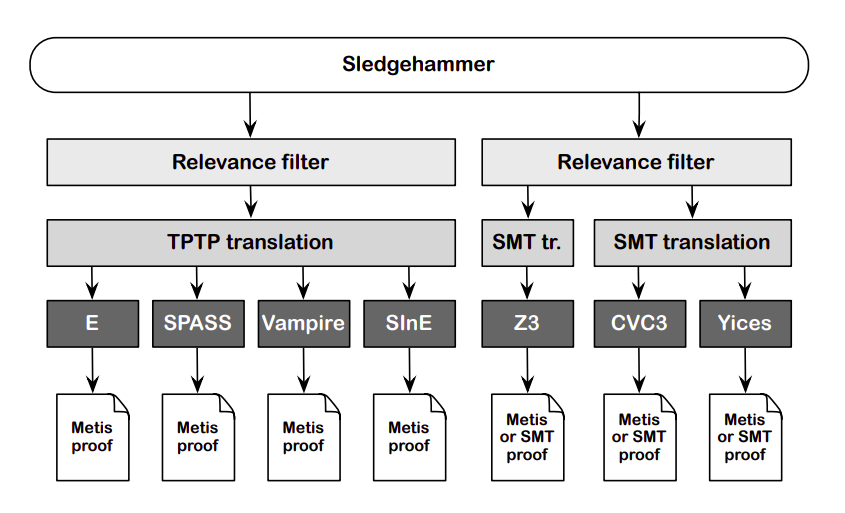
\includegraphics[width=\textwidth]{Sledgehammer_arquitecture.png}
	\caption{Arquitectura de Sledgehammer. Extraída de~\cite{proof_and_disproof}.}\label{fig:Sledgehammer_arquitecture.}
\end{figure}

Idealmente, los probadores de terceros se incluyen en un paquete con Isabelle y están listos para usarse sin necesidad de configuración. Isabelle incluye ejecutables CVC3, E, SPASS y Z3 para las principales plataformas de hardware; los usuarios pueden descargar Yices y Vampire, cuyas licencias prohíben la redistribución, pero la mayoría simplemente ejecuta Vampire de forma remota en SystemOnTPTP.\@

Los servidores remotos son ideales para la búsqueda de pruebas, al menos cuando están funcionando y el usuario tiene acceso a Internet. También ayudan a distribuir la carga: a menos que la máquina del usuario posea un procesador de ocho núcleos procesador, sería imprudente lanzar cuatro probadores de resolución y tres solvers SMT y esperar que la interfaz de usuario de Isabelle siga respondiendo. La invocación paralela de probadores es invaluable: ejecutar E, SPASS y Vampire juntos durante cinco segundos resuelve tantos problemas como ejecutar un solo probador durante dos minutos~\cite{sledgehammer_judgement_day}.

\subsubsection{Reconstruyendo la prueba}

Para probadores de resolución, Sledgehammer realiza una reconstrucción de prueba ejecutando el probador de resolución integrado de Isabelle, Metis, brindando la breve lista de hechos utilizados en la prueba encontrada por el prover. Dado solo unos pocos hechos, Metis generalmente tiene éxito en milisegundos. Dado que Metis tiene que volver a encontrar la prueba, los provers externos se utilizan esencialmente como filtros de relevancia de gran precisión.

Las pruebas generadas usualmente requieren una edición a posteriori para volverlas sintácticamente correctas. Las nuevas actualizaciones siempre realizan esfuerzos para hacer que el resultado generado sea más robusto y conciso.

Con respecto a SMT, las pruebas que no involucran razonamiento aritmético generalmente pueden ser reproducidas por Metis; de lo contrario, se admite la reproducción de la prueba, paso a paso, para Z3. Mientras que CVC3 e Yices se pueden invocar como oráculos. La repetición de la prueba Z3 se basa en gran medida en los procedimientos de decisión aritmética, simplificador y probador de tipo tableau de Isabelle.

\subsubsection{Minizando la prueba}

Los probadores externos usualmente usan muchos más hechos de los necesarios. La herramienta de minimización de Sledgehammer toma el conjunto de hechos usados retornados por un prover e invoca repetidamente al mismo con subconjuntos de los hechos para encontrar un conjunto mínimo.

Dependiendo del número de hechos iniciales, se basa en un algoritmo lineal `naive' que intenta eliminar un hecho a la vez o en un algoritmo binario que biseca recursivamente los hechos~\cite{sledgehammer_judgement_day}.

La minimización frecuentemente mejora el rendimiento y la tasa de éxito de Metis, y al mismo tiempo elimina el desorden de las formalizaciones de Isabelle. Para algunos provers, es difícil o imposible extraer la lista de hechos usados de la prueba; la minimización es entonces la única opción. Por ejemplo, las pruebas detalladas devueltas por CVC3 siempre se refieren a todos los hechos, sean realmente necesarios o no, y no existe un criterio fácil para aislar los hechos necesarios.

\subsection{Quickcheck: Generación de contraejemplos}

Los métodos de prueba de Isabelle y Sledgehammer son efectivos frente a conjeturas válidas, pero dada una conjetura inválida, normalmente no detectan la invalidez de la misma, y mucho menos producen un contraejemplo relevante.

Aquí es donde entra en escena Quickcheck. Quickcheck se modeló originalmente a partir de la herramienta QuickCheck para Haskell~\cite{quickcheck_haskell}, que prueba las propiedades proporcionadas por el usuario de un programa Haskell para valores generados aleatoriamente. Recientemente Quickcheck se ha ampliado con pruebas exhaustivas y basadas en restricciones como complemento a las pruebas aleatorias.

Las pruebas exhaustivas verifican la fórmula para cada posible conjunto de valores hasta un límite dado, y por lo tanto encuentran contraejemplos que las pruebas aleatorias podrían pasar por alto. La reducción puede ser más precisa y eficiente que los otros dos enfoques porque considera la fórmula simbólicamente, en lugar de probar un conjunto finito de valores fundamentales. Gracias a un análisis de flujo de datos estáticos, inspirado en la programación lógica, Quickcheck deriva generadores de datos de prueba que tienen en cuenta las premisas para ayudar a evitar los casos de prueba vacíos que afectan a la mayoría de las herramientas de prueba de especificaciones.


\section{Programando y probando en Isabelle/HOL}

Esta sección introduce a HOL como un lenguaje de programación funcional y muestra como probar propiedades de programas funcionales mediante inducción~\cite{prog-prove-isabelle}.

\subsection{Definiciones básicas}

\subsubsection{Tipos, términos y fórmulas}

HOL es considerado una lógica tipada, cuyo sistema de tipos se asemeja al de los lenguajes de programación funcional. Esto implica la existencia de:

\begin{itemize}
	\item \textbf{Tipos base}: Los cuales están conformados por \texttt{bool}, el tipo de valor de verdad, \texttt{nat}, el tipo de los números naturales ($\mathbb{N}$), e \texttt{int}, el tipo de los números enteros ($\mathbb{Z}$).
 	\item \textbf{Constructores de tipo}: En particular \texttt{list}, el tipo de listas y \texttt{set}, el tipo de conjuntos. Los constructores de tipos se escriben como posfijos, es decir, después de sus argumentos. Por ejemplo, \texttt{nat list} es el tipo de listas cuyos elementos son números naturales.
  	\item \textbf{Funciones}: Denotadas con $\Rightarrow$.
  	\item \textbf{Variables de tipo}: Denotadas por $'a$, $'b$, etc., como en ML~\cite{ML_programming_language}.
\end{itemize}

Los \textbf{términos} se forman como en la programación funcional, aplicando funciones a los argumentos. Si $f$ es una función de tipo $\tau_1 \Rightarrow \tau_2$ y $t$ es un término de tipo $\tau_1$ entonces $f\ t$ es un término de tipo $\tau_2$. Escribimos $t :: \tau$ para indicar que el término $t$ tiene tipo $\tau$. Los términos abarcan también abstracciones lambda. Por ejemplo $\lambda x.\ x$ es la función identidad.

Las \textbf{fórmulas} son términos de tipo \textit{bool}. Entre ellas se encuentran las constantes básicas \texttt{True} y \texttt{False} y los conectores lógicos usuales (en orden decreciente de precedencia): $\neg,\ \vee,\ \wedge,\ \rightarrow$.

La \textbf{igualdad} está disponible en la forma de la función infijo \textbf{=}, del tipo $'a \Rightarrow 'b \Rightarrow  bool$. También funciona para formulas, donde significa `si o solo si'.

Los \textbf{cuantificadores} se escriben como $\forall\ x.\ P$ y $\exists\ x.\ P$.

Isabelle automáticamente computa el tipo de cada variable en un término. Esto se conoce popularmente como inferencia de tipos. A pesar de la inferencia de tipos, en ocasiones es necesario agregar el tipo explícito a una variable o término. La sintaxis es $t :: \tau$ como en $m + (n::nat)$. Las anotaciones explicitas de tipos son especialmente necesarias para desambiguar términos que incluyen funciones sobrecargadas como $+$.

Finalmente nos encontramos con el cuantificador universal $\bigvee$ y la implicación $\Longrightarrow$. Estos son parte del framework Isabelle, no de HOL.\@

\subsection{Teorías}

Una teoría es una colección de tipos, funciones y teoremas, similar a un módulo en un lenguaje de programación. Todo el contenido que escribamos en Isabelle debe pertenecer a una teoría. El formato general de una teoría T es:

\begin{lstlisting}[style=Isabelle]
theory $T$
imports $T_1, \cdots, T_n$
begin
$\text{definitions, theorems and proofs}$
end
\end{lstlisting}

donde $T_1 \ldots T_n$ son los nombres de teorías existentes en las que $T$ está basado. Se dice que $T_i$ son las teorías padre de $T$. Todo lo definido en los padres de $T$ (y los padres de sus padres, recursivamente) es visible automáticamente. Cada teoría $T$ debe estar guardada en un archivo llamado \texttt{T.thy}.

Ademas de las teorías que incluye por defecto la distribución de Isabelle/HOL\footnote{\href{https://isabelle.in.tum.de/library/HOL}{https://isabelle.in.tum.de/library/HOL}}, se encuentra disponible un archivo de pruebas formales (\href{https://isa-afp.org}{https://isa-afp.org}), el cual está en constante crecimiento y en el que cualquier persona puede contribuir.


\subsubsection{Comillas}
La definición textual de una teoría sigue una sintaxis especifica incluyendo keywords como \textbf{begin} y \textbf{datatype}. En esta sintaxis están embebidos los tipos y fórmulas de HOL.\@ Para distinguir los dos niveles, todo lo específico de HOL (términos y tipos) debe estar entre comillas: \texttt{"\ldots"}. Las comillas alrededor de un único identificador se pueden eliminar. Cuando Isabelle imprime un mensaje de error de sintaxis, se refiere a la sintaxis HOL como la sintaxis interna y al lenguaje teórico adjunto como la sintaxis externa.% chktex 18 // intencionalmente usando "" en lugar de ``''

\subsubsection{Estado de la prueba} 

En una instalación habitual de Isabelle\footnote{\href{https://isabelle.in.tum.de/}{https://isabelle.in.tum.de/}}, con el cursor en un `lemma' o `theorem', es posible ver en la pestaña `state', los subgoals y estado parcial de nuestra prueba en proceso.

\begin{figure}[H]
	\centering
    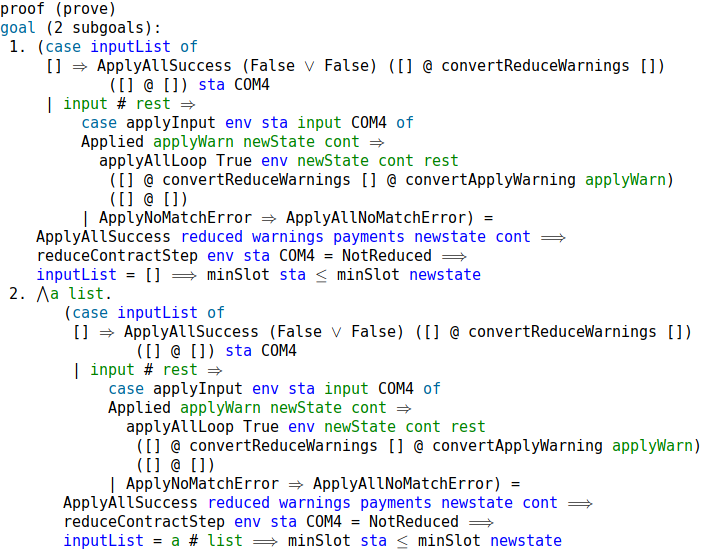
\includegraphics[width=0.7\textwidth]{Proof_state_isabelle.png}
	\caption{Pantalla de `status' para una prueba en proceso de la sintaxis de Marlowe.}\label{fig:Proof_state}
\end{figure}


\subsection{Algunos tipos y pruebas básicas}

En esta sección detallaremos los tipos \textit{bool}, \textit{nat} y \textit{list}, los más importantes y utilizados en Isabelle/HOL.\@ Mostremos algunos ejemplos de pruebas sencillas y las probaremos con inducción y simplificación.

\subsubsection{bool}

Este tipo esta predefinido mediante:

\begin{lstlisting}[style=Isabelle]
datatype bool = True | False
\end{lstlisting}

El mismo cuenta con los valores \texttt{True} y \texttt{False} y algunas funciones predefinidas,\\ como:  $\neg,\ \vee,\ \wedge,\ \rightarrow$, etc. El siguiente ejemplo muestra como puede definirse la conjunción lógica (conocida también como intersección en teoría de conjuntos) mediante `\textit{pattern matching}':

\begin{lstlisting}[style=Isabelle]
  fun conj :: "bool $\Rightarrow$ bool $\Rightarrow$ bool" where
  "conj True True = True" |
  "conj _ _ = False"}
\end{lstlisting}

Las definiciones de datatype y funciones siguen la sintaxis de lenguajes de programación funcional.

\subsubsection{nat}
Los números naturales y otros datatypes predefinidos.

\begin{lstlisting}[style=Isabelle]
datatype nat = 0 | Suc nat
\end{lstlisting}

Todos los valores de tipo \texttt{nat} son generados por los constructores \texttt{0} y \texttt{Suc}. Por lo tanto, los valores de tipo nat son \texttt{0}, \texttt{Suc 0}, \texttt{Suc (Suc 0)}, etc. Algunas de las funciones predefinidas son: +, *, $\leq$, etc. A continuación, vemos como podríamos definir nuestra propia operación de suma:

\begin{lstlisting}[style=Isabelle]
  fun add :: "nat $\Rightarrow$ nat $\Rightarrow$ nat" where
  "add 0 n = n" |
  "add (Suc m) n = Suc(add m n)"
\end{lstlisting}

Y a continuación vemos una prueba de \texttt{add m 0 = m}:
\begin{lstlisting}[style=Isabelle]
  lemma add_02: "add m 0 = m"
  apply(induction m)
  apply(auto)	  
  done
\end{lstlisting}

La palabra reservada \texttt{lemma} comienza la prueba y le da al lema un nombre, por ejemplo `\texttt{add\_02}'. Las propiedades definidas recursivamente suelen ser probadas por inducción en la mayoría de las ocasiones. El commando \texttt{apply (induction m)} le indica a Isabelle que debe comenzar una prueba por inducción, en la variable \texttt{m}. Como respuesta, va a mostrar el siguiente `estado de prueba':

\begin{enumerate}
	\item \texttt{add 0 0 = 0}
	\item $\bigwedge$ \texttt{m.\ add m 0 = m} $\Longrightarrow$ \texttt{add (Suc m) 0 = Suc m}	
\end{enumerate}

Las lineas numeradas son conocidas como subgoals. El primer subgoal es el caso base, y el segundo es el paso inductivo. El prefijo $\bigwedge$ \texttt{m. }es la forma en la que Isabelle nos comunica ``para un m arbitrario, pero fijo''. El símbolo $\Longrightarrow$ separa las suposiciones de la conclusión. El comando \texttt{apply (auto)} (mencionado por primera vez en~\ref{sec:auto}) le indica a Isabelle que intente probar todos los subgoals automáticamente, en este caso simplemente mediante simplificación. Debido a la sencillez de ambos subgoals, Isabelle puede manejarlos con las teorías incluidas por defecto. 

El caso base \texttt{add 0 0 = 0} se prueba por la definición de \texttt{add} y el paso inductivo es casi tan simple: \texttt{add (Suc m) 0 = Suc (add m 0) = Suc m} usando la definición de \texttt{add} y la hipótesis inductiva respectivamente. En resumen, ambas `sub-pruebas' se basan en la simplificación mediante la definición y la hipótesis inductiva. Como resultado de la keyword `\texttt{done}', Isabelle asocia el lema a su identificador.

De ahora en más dicho lema podría ser utilizado como algún paso de prueba por lemas subsiguientes.

\subsubsection{Listas}

Las listas ya están predefinidas por Isabelle\footnote{Dicha definición puede ser encontrada en \href{https://isabelle.in.tum.de/library/HOL/HOL/List.html}{https://isabelle.in.tum.de/library/HOL/HOL/List.html}}, pero su definición puede ser simplificada como:

\begin{lstlisting}[style=Isabelle]
datatype 'a list = Nil | Cons 'a "'a list"
\end{lstlisting}

\begin{itemize}
	\item La lista \texttt{'a list} es el conjunto de listas con elementos de tipo \texttt{'a}. Debido a que \texttt{'a} es una variable de tipo, las listas son de hecho polimórficas: Los elementos de una lista pueden ser de tipo arbitrario (pero todos los elementos deben compartir el tipo).

	\item Las listas tienen dos constructores: \texttt{Nil}, la lista vacía y \texttt{Cons}, que agrega un elemento de tipo \texttt{'a} en el comienzo de la misma (de tipo \texttt{'a list}). Esto provoca que todas las listas sean de la forma \textit{\texttt{Nil}}, \textit{\texttt{Cons x Nil}} o \textit{\texttt{Cons x (Cons y Nil)}}, etc.
	
\end{itemize}


%##########################
% Desarrollo: verificación de contratos financieros usando Isabelle
%##########################

\chapter[Verificación de contratos financieros en Isabelle]{Desarrollo: Verificación de contratos financieros usando Isabelle}
\section{Escritura de contratos ACTUS para Cardano}

En esta sección, veremos como se desarrolló la escritura de tres contratos ACTUS para la blockchain Cardano, en conjunto con IOHK.\@

Cabe destacar que durante esta tarea, tuve la colaboración de Yves Hauser\footnote{\href{https://iohk.io/en/team/yves-hauser}{https://iohk.io/en/team/yves-hauser}}, con quien conversamos sobre decisiones de diseño e implementación de los contratos correspondientes. Yves fue el responsable de integrar mis cambios a la rama \textit{master} del repositorio de \texttt{marlowe-cardano} \cite{marlowe-cardano-github}. %chktex 2

\newpage
\subsection{Descripción de la estructura del proyecto}\label{sec:estructura}

En la siguiente sub-sección, describiremos brevemente algunos de las entidades relevantes para la implementación de un contrato. Para eso, es importante conocer la estructura de archivos del mismo, junto con la responsabilidad de algunos de ellos.

\begin{figure}[H]
\begin{tikzpicture}
	\draw[color=black!60!white]
	\FTdir(\FTroot,root,.){       % root: parent = \FTroot
	  \FTdir(root,Language,Language){       % normal dir: (parentID, currentID, label)
          \FTdir(Language,Marlowe,Marlowe){                    
              \FTdir(Marlowe,ACTUS,ACTUS){                    
                  \FTdir(ACTUS,Domain,Domain){
                      \FTfile(Domain,BusinessEvents.hs)
                      \FTfile(Domain,ContractState.hs)
                      \FTfile(Domain,ContractTerms.hs)
                      \FTfile(Domain,Ops.hs)
                      \FTfile(Domain,Schedule.hs)
                  }
                  ++(0,-0.5em)                
                  \FTdir(ACTUS,Generator,Generator){
                      \FTfile(Generator,Analysis.hs)
                      \FTfile(Generator,Generator.hs)
                      \FTfile(Generator,GeneratorFs.hs)
                      \FTfile(Generator,GeneratorStatic.hs)
                      \FTfile(Generator,MarloweCompat.hs)
                  }
                  ++(0,-0.5em)                
                  \FTdir(ACTUS,Model,Model){
                      \FTfile(Model,Applicability.hs)
                      \FTfile(Model,ContractSchedule.hs)
                      \FTfile(Model,Payoff.hs)
                      \FTfile(Model,StateInitialization.hs)
                      \FTfile(Model,StateTransition.hs)
                  }
                  ++(0,-0.5em)                
                  \FTdir(ACTUS,Utility,Utility){
                      \FTdir(Utility,ANN,ANN){
                          \FTfile(ANN,Annuity.hs)
                      }
                      \FTfile(Utility,DateShift.hs)
                      \FTfile(Utility,ScheduleGenerator.hs)
                      \FTfile(Utility,YearFraction.hs)
                  }
              }
          }
      }
    };
\end{tikzpicture}
\caption{Árbol de archivos en el repositorio del lenguaje Marlowe. Extraído de~\cite{marlowe-language-repo}.}\label{fig:Marlowe_dirtree}
\end{figure}

Para comenzar, podemos observar los cuatro directorios principales: \texttt{Domain}, \texttt{Generator}, \texttt{Model} y \texttt{Utility}. En los mismos es posible encontrar el código necesario para modelar los contratos ACTUS, generar contratos el código de los mismos en Marlowe o en Haskell para luego ser ejecutados.

\subsubsection{Domain}

El mismo está conformado por los archivos que modelan el dominio de los contratos ACTUS.\@

\begin{tikzpicture}
	\draw[color=black!60!white]
    \FTdir(\FTroot,Domain,Domain){
        \FTfile(Domain,BusinessEvents.hs)
        \FTfile(Domain,ContractState.hs)
        \FTfile(Domain,ContractTerms.hs)
        \FTfile(Domain,Ops.hs)
        \FTfile(Domain,Schedule.hs)
    };
\end{tikzpicture}

A lo largo de los mismos, se ven definiciones de tipos necesarios en ACTUS.\@Como por ejemplo: `EventType' o `RiskFactorsPoly' en \texttt{BusinessEvents.hs} o `ContractStatePoly' en\\ \texttt{ContractState.hs}.

A continuación vemos algunos fragmentos de algunas definiciones de tipos:

\begin{lstlisting}[style=Haskell-cardano, caption=Algunos tipos de eventos.]
{-| ACTUS event types
    https://github.com/actusfrf/actus-dictionary/blob/master/actus-dictionary-event.json
-}
data EventType =
      IED  -- ^ Initial Exchange
    | FP   -- ^ Fee Payment
    | PR   -- ^ Principal Redemption
    | PD   -- ^ Principal Drawing
    | PY   -- ^ Penalty Payment
    | PP   -- ^ Principal Prepayment (unscheduled event)
    | IP   -- ^ Interest Payment
    | IPFX -- ^ Interest Payment Fixed Leg
    | IPFL -- ^ Interest Payment Floating Leg
    | IPCI -- ^ Interest Capitalization
    | CE   -- ^ Credit Event

    [...]

    | MD   -- ^ Maturity
    | XD   -- ^ Exercise
    | STD  -- ^ Settlement
    | PI   -- ^ Principal Increase
    | AD   -- ^ Monitoring
\end{lstlisting}

\begin{lstlisting}[style=Haskell-cardano, caption=Contract state poly.]

{-| ACTUS contract states are defined in
    https://github.com/actusfrf/actus-dictionary/blob/master/actus-dictionary-states.json
-}
data ContractStatePoly a = ContractStatePoly
  {
    tmd   :: Maybe LocalTime -- ^ Maturity Date (MD): The timestamp as per which the contract matures according to the initial terms or as per unscheduled events
  , nt    :: a               -- ^ Notional Principal (NT): The outstanding nominal value
  , ipnr  :: a               -- ^ Nominal Interest Rate (IPNR) : The applicable nominal rate
  , ipac  :: a               -- ^ Accrued Interest (IPAC): The current value of accrued interest
  , ipac1 :: Maybe a         -- ^ Accrued Interest (IPAC1): The current value of accrued interest of the first leg
  , ipac2 :: Maybe a         -- ^ Accrued Interest (IPAC2): The current value of accrued interest of the second leg
  , ipla  :: Maybe a         -- ^ Last Interest Period
  , feac  :: a               -- ^ Fee Accrued (FEAC): The current value of accrued fees
  , nsc   :: a               -- ^ Notional Scaling Multiplier (SCNT): The multiplier being applied to principal cash flows
  , isc   :: a               -- ^ InterestScalingMultiplier (SCIP): The multiplier being applied to interest cash flows
  , prf   :: PRF             -- ^ Contract Performance (PRF)
  , sd    :: LocalTime       -- ^ Status Date (MD): The timestamp as per which the state is captured at any point in time
  , prnxt :: a               -- ^ Next Principal Redemption Payment (PRNXT): The value at which principal is being repaid
  , ipcb  :: a               -- ^ Interest Calculation Base (IPCB)
  , xd    :: Maybe LocalTime -- ^ Exercise Date (XD)
  , xa    :: Maybe a         -- ^ Exercise Amount (XA)
  }
\end{lstlisting}


También es posible ver tipos relacionados a características de un contrato, como `ContractType', `ContractRole', `DayCountConvention', `BusinessDayConvention', etc en \texttt{ContractTerms.hs}.

A continuación vemos algunos fragmentos de algunas definiciones de los mismos:

\begin{lstlisting}[style=Haskell-cardano, caption=Tipos de contrato.]
-- |ContractType
data CT = PAM   -- ^ Principal at maturity
        | LAM   -- ^ Linear amortizer
        | NAM   -- ^ Negative amortizer
        | ANN   -- ^ Annuity
        | STK   -- ^ Stock
        | OPTNS -- ^ Option
        | FUTUR -- ^ Future
        | COM   -- ^ Commodity
        | CSH   -- ^ Cash
        | CLM   -- ^ Call Money
        | SWPPV -- ^ Plain Vanilla Swap
        | CEG   -- ^ Guarantee
        | CEC   -- ^ Collateral
\end{lstlisting}

\begin{lstlisting}[style=Haskell-cardano, caption=Algunos tipos de roles de contrato.]
-- |ContractRole
data CR = CR_RPA -- ^ Real position asset
        | CR_RPL -- ^ Real position liability
        | CR_CLO -- ^ Role of a collateral
        | CR_CNO -- ^ Role of a close-out-netting
        | CR_COL -- ^ Role of an underlying to a collateral
        | CR_LG  -- ^ Long position
        | CR_ST  -- ^ Short position
        | CR_BUY -- ^ Protection buyer
        | CR_SEL -- ^ Protection seller

        [...]
\end{lstlisting}


\begin{lstlisting}[style=Haskell-cardano, caption=Tipos de convención sobre días laborables.]
-- |BusinessDayConvention
data BDC = BDC_NULL -- ^ No shift
         | BDC_SCF  -- ^ Shift/calculate following
         | BDC_SCMF -- ^ Shift/calculate modified following
         | BDC_CSF  -- ^ Calculate/shift following
         | BDC_CSMF -- ^ Calculate/shift modified following
         | BDC_SCP  -- ^ Shift/calculate preceding
         | BDC_SCMP -- ^ Shift/calculate modified preceding
         | BDC_CSP  -- ^ Calculate/shift preceding
         | BDC_CSMP -- ^ Calculate/shift modified preceding
\end{lstlisting}


\subsubsection{Generator}

En este directorio se implementan los diferentes generadores y compatibilidad hacia el lenguaje Marlowe.

\begin{tikzpicture}
    \draw[color=black!60!white]
    \FTdir(\FTroot,Generator,Generator){
        \FTfile(Generator,Analysis.hs)
        \FTfile(Generator,Generator.hs)
        \FTfile(Generator,GeneratorFs.hs)
        \FTfile(Generator,GeneratorStatic.hs)
        \FTfile(Generator,MarloweCompat.hs)
    };
\end{tikzpicture}


En el archivo \texttt{Analysis.hs}, se definen las funciones:

\begin{itemize}
    \item \texttt{genProjectedCashflows}
    \item \texttt{genCashflow}
    \item \texttt{genSchedules}
    \item \texttt{genStates}
    \item \texttt{genPayoffs}
\end{itemize}

Las mismas, como sus nombres lo indican, generan los flujos de dinero proyectados, flujos de dinero, cronogramas, estados y pagos respectivamente. Los flujos de dinero pueden ser utilizados para generar los pagos en un contrato en Marlowe.

En \texttt{GeneratorStatic.hs}, mediante la función \texttt{genFsContract} genera un contrato en Marlowe a partir de los términos de contrato ACTUS.\@En \texttt{genFsContract}, los `risk factors' son agregados al contrato en Marlowe, en otras palabras, será `observado' durante la vida del mismo.

La función \texttt{genStaticContract}, en \texttt{GeneratorStatic.hs}, valida que los términos del contrato sean correctos, para poder genera un contrato en Marlowe donde los `risk factors' sean conocidos de antemano. Esta restricción desencadena en contratos que solo consisten de transacciones, i.e. \texttt{Deposit} y \texttt{Pay}.

Con respecto a \texttt{MarloweCompat.hs}, contiene algunas funciones auxiliares y la función\\ \texttt{toMarlowe}, que se ocupa de recibir los términos del contrato en haskell y realizar la traducción a términos del contrato en Marlowe. 

A continuación se muestra el fragmento inicial de la misma:


\begin{lstlisting}[style=Haskell-cardano, caption=Comienzo de la función \texttt{toMarlowe}.]
toMarlowe :: ContractTerms -> ContractTermsMarlowe
toMarlowe ct =
  ContractTermsPoly
    { contractId = contractId ct,
      contractType = contractType ct,
      contractStructure = map trans (contractStructure ct),
      contractRole = contractRole ct,
      settlementCurrency = settlementCurrency ct,
      initialExchangeDate = initialExchangeDate ct,
      dayCountConvention = dayCountConvention ct,
      scheduleConfig = scheduleConfig ct,
      statusDate = statusDate ct,
      contractPerformance = contractPerformance ct,
      creditEventTypeCovered = creditEventTypeCovered ct,

      [...]
\end{lstlisting}

\subsubsection{Model}

En este directorio se encuentran los archivos que modelan la lógica expuesta por el estándar ACTUS, tales como Schedule, Inicialización de variables de estado y funciones de transición de estado y de pago.

\begin{tikzpicture}
    \draw[color=black!60!white]
    \FTdir(\FTroot,Model,Model){
        \FTfile(Model,Applicability.hs)
        \FTfile(Model,ContractSchedule.hs)
        \FTfile(Model,Payoff.hs)
        \FTfile(Model,StateInitialization.hs)
        \FTfile(Model,StateTransition.hs)
    };
\end{tikzpicture}

Las reglas de aplicabilidad\footnote{Especificadas en \href{https://www.actusfrf.org/aplicability}{https://www.actusfrf.org/aplicability}} son definidas, para cada tipo de contrato. Las reglas revisan la consistencia de los atributos de contrato, para los términos de un contrato ACTUS dado. Si los términos son validados satisfactoriamente, se espera que el contrato sea significativo y flujos de dinero puedan ser proyectados. Dicha condición es chequeada en \texttt{Applicability.hs}

Con respecto a \texttt{ContractSchedule.hs}, \texttt{Payoff.hs}, \texttt{StateInitialization.hs} y\\ \texttt{StateTransition.hs}, se ocupan de ajustar el cronograma, los pagos, inicializar las variables de estado, y las transiciones sobre las mismas.

Como ejemplo, puede verse reflejado el cambio de estado para el contrato PAM y evento IPCI (Interest Capitalization) en parte de la implementación de la función \texttt{stateTransition}:

\begin{lstlisting}[style=Haskell-cardano, caption=Parte de la función que modela la transicción de estados.]
        [...]
        ------------------------------------
        -- Interest Capitalization (IPCI) --
        ------------------------------------
        -- STF_IPCI_PAM
        -- STF_IPCI_CLM
        stf
          IPCI
          rf
          ct@ContractTermsPoly
            { contractType,
              dayCountConvention = Just dcc,
              maturityDate
            }
          st@ContractStatePoly
            { ..
            } | contractType `elem` [PAM, CLM] =
            let y_sd_t = _y dcc sd t maturityDate
                st' = stf IP rf ct st
             in st'
                  { nt = nt + ipac + y_sd_t * nt * ipnr
                  }
        [...]
\end{lstlisting}

La misma refleja las variables siendo ajustadas de acuerdo al estándar:

\begingroup
\fontsize{9pt}{9pt}\selectfont


\begin{functions}{PAM}
	IPCI & 0.0
	& {$\begin{aligned}
					\svar{Nt}{t^+}   & = \svar{Nt}{t^-} + \svar{Ipac}{t^-} + \yfr{\svar{Sd}{t^-}}{t}\svar{Nt}{t^-}\svar{Ipnr}{t^-}                                         \\
					\svar{Ipac}{t^+} & = 0.0                                                                                                                               \\
					\svar{Feac}{t^+} & = \begin{cases} \svar{Feac}{t^-} + \yfr{\svar{Sd}{t^-}}{t}\svar{Nt}{t^-}\attr{FER} & \text{if} \quad \attr{FEB}=\text{'N'} \\
              \frac{\yfr{t^{FP-}}{t}}{\yfr{t^{FP-}}{t^{FP+}}}\sgn\attr{FER}      & \text{else}\end{cases} \\
					\svar{Sd}{t^+}   & = t\end{aligned}$} \par
	with\par
	{$\begin{aligned}
				t^{FP-} & = \sup t \in \vec{t}^{FP}\mid t<t_0 \\
				t^{FP+} & = \inf t \in \vec{t}^{FP}\mid t>t_0\end{aligned}$} \\
	\hline
\end{functions}
\endgroup




\subsubsection{Utility}

En este directorio se encuentran algunos archivos con funciones que se utilizan para aislar la lógica del calculo de fechas, que suele tornarse complejo y repetitivo durante los contratos.

\begin{tikzpicture}
	\draw[color=black!60!white]
	\FTdir(\FTroot,Utility,Utility){ 
        \FTdir(Utility,ANN,ANN){
            \FTfile(ANN,Annuity.hs)
        }
        \FTfile(Utility,DateShift.hs)
        \FTfile(Utility,ScheduleGenerator.hs)
        \FTfile(Utility,YearFraction.hs)
    };
\end{tikzpicture}

\sloppy Funciones para calcular determinadas fechas, para cada tipo de convención de día hábil, son extraídas en el módulo \texttt{DateShift.hs}, como por ejemplo: \texttt{applyBDC}, \texttt{getPreceedingBusinessDay}, \texttt{moveToEndOfMonth}, etc.

\subsection{Metodología de escritura de un Contrato ACTUS en Cardano}

Para poder escribir un contrato, es necesario revisar los eventos que disparan acciones del contrato, las mismas están especificadas en~\cite{ACTUS_Techspecs}, también esta disponible una implementación oficial en Java de los mismos, en la cual es posible basarse. Es conveniente utilizar ambos, ya que se reduce el esfuerzo de implementación en Haskell cuando se cuenta con ellos.

Para cada contrato, se agregan casos a los archivos vistos previamente en~\ref{sec:estructura}, tanto para el modelo como para el dominio. En algunos casos, quizas sea necesario agregar alguna función en Utility.

Con repecto a la implementación en Java, la misma no es pública, pero con fines de la implementación de los siguientes contratos, me fue otorgado por parte de IOHK un token de acceso para poder clonarla y usarla durante la implementación.

Todas las implementaciones son testeadas usando algunos ejemplos\footnote{Disponibles en \href{https://github.com/input-output-hk/marlowe-cardano/blob/main/marlowe-actus/test/Spec/Marlowe/ACTUS/Examples.hs}{https://github.com/input-output-hk/marlowe-cardano/blob/main/marlowe-actus/test/Spec/Marlowe/ACTUS/Examples.hs}}, así como también la batería de tests propuestos por ACTUS~\cite{ACTUS_Tests}.

En los tests propuestos por ACTUS, un conjunto de términos de contrato y eventos disparadores son provistos, y se espera que ciertos eventos sean generados por la implementación. Debido a que ACTUS es agnostica a la misma, los test solo reflejan los eventos esperados, pero no como serán ejectutados en la plataforma (en este caso, en la blockchain Cardano).

A continuación se muestra un test de ejemplo para el contrato COM, provisto por ACTUS:\@


\begin{lstlisting}[style=Haskell-cardano, caption=Test propuesto por ACTUS para el contrato COM. Se pueden ovservar tanto los términos como eventos observados y los eventos que se esperá que la implementación genere.]
"com04": {
        "identifier": "com04",
        "terms": {
            "contractType": "COM",
            "contractID": "com04",
            "statusDate": "2014-12-30T00:00:00",
            "contractDealDate": "2014-12-15T00:00:00",
            "purchaseDate": "2015-03-30T00:00:00",
            "priceAtPurchaseDate": "700",
            "terminationDate": "2016-02-20T00:00:00",
            "priceAtTerminationDate": "900",
            "contractRole": "RPL",
            "currency": "GBP",
            "marketValueObserved": "100",
            "quantity": "3",
            "unit": "BRL"
        },
        "to": "2016-03-30T00:00:00",
        "dataObserved": {

        },
        "eventsObserved": [

        ],
        "results": [
            {
                "eventDate": "2015-03-30T00:00:00",
                "eventType": "PRD",
                "payoff": 2100,
                "notionalPrincipal": 0,
                "nominalInterestRate": 0,
                "accruedInterest": 0,
                "currency": "GBP"
            },
            {
                "eventDate": "2016-02-20T00:00:00",
                "eventType": "TD",
                "payoff": -2700,
                "notionalPrincipal": 0,
                "nominalInterestRate": 0,
                "accruedInterest": 0,
                "currency": "GBP"
            }
        ]
    }
\end{lstlisting}

Dicho \texttt{json} es procesado en \href{https://github.com/input-output-hk/marlowe-cardano/blob/main/marlowe-actus/test/Spec/Marlowe/ACTUS/TestFramework.hs}{TestFramework.hs}, donde se parsea la entrada, se ejectura el generador, y se comparan los campos del json inicial con los del objeto generado por la implementación.

Por otro lado, podemos ver el test de ejemplo agregado para el contrato COM 

\begin{lstlisting}[style=Haskell-cardano, caption=Test de ejemplo escrito durante el desarrollo de la tesis para el contrato COM.]
-- |ex_com1 defines a contract of type COM
ex_com1 :: IO ()
ex_com1 =
  contractFromFile "test/Spec/Marlowe/ACTUS/ex_com1.json"
    >>= either msg run
  where
    msg err = putStr err
    run ct = case genFsContract defaultRiskFactors (toMarlowe ct) of
      Failure _ -> assertFailure "Terms validation should not fail"
      Success contract ->
          let principal = NormalInput . IDeposit (Role "party") "party" ada
              out =
                computeTransaction
                  ( TransactionInput
                      (0, 0)
                      [ principal 1400
                      ]
                  )
                  (emptyState 0)
                  contract
           in case out of
                Error _ -> assertFailure "Transactions are not expected to fail"
                TransactionOutput txWarn txPay _ con -> do
                  assertBool "Contract is in Close" $ con == Close
                  assertBool "No warnings" $ null txWarn

                  assertBool "total payments to party" (totalPayments (Party "party") txPay == 0)
                  let tc = totalPayments (Party "counterparty") txPay
                  assertBool ("total payments to counterparty: " ++ show tc) (tc == 1400)

contractFromFile :: FilePath -> IO (Either String ContractTerms)
contractFromFile f = eitherDecode <$> B.readFile f
\end{lstlisting}

El mismo se ocupa de tomar los términos del contrato de un archivo \texttt{ex\_com1.json} (de sintaxis similar a los de ACTUS) y ejecutar el generador. Luego valida que las transacciones computadas sean las esperadas, así como también que los balances en las wallets corresponientes sean consistentes.

% Contrato COM
\subsection{Contrato COM (Commodity)}

Según su descripción en~\cite{ACTUS_Dictionary}:

\begin{quote} 
``Este contrato no es de tipo financiero en el sentido estricto. Sin embargo, realiza el seguimiento de los movimientos de commodities como el petroleo, gas o incluso viviendas. Dichas commodities pueden utilizarse servir como garantía subyacente de futuros en materias primas, garantías o simplemente posiciones de activos.''
\end{quote}

\subsubsection{Especificación técnica}

A continuación adjunto la especificación técnica del contrato COM~\cite{ACTUS_Techspecs}:

% ---------------------- table: com schedule ----------------------
\begingroup
\fontsize{9pt}{9pt}\selectfont
\begin{schedule}{COM}
	AD & & Same as PAM \\
	\hline
	PRD & & Same as STK \\
	\hline
	TD & & Same as STK \\
\end{schedule}
\endgroup

% ---------------------- table: com states ----------------------
\begingroup
\fontsize{9pt}{9pt}\selectfont
\begin{states}{COM}
	$\svar{Sd}{}$ & & Same as STK \\
\end{states}
\endgroup

% ---------------------- table: com functions ----------------------
\begingroup
\fontsize{9pt}{9pt}\selectfont
\begin{functions}{COM}
	AD & \pof{AD}{PAM} & \stf{AD}{STK} \\
	\hline
	PRD & \pof{PRD}{STK} & \stf{PRD}{STK} \\
	\hline
	TD & \pof{PRD}{STK} & \stf{PRD}{STK} \\
\end{functions}
\endgroup

El contrato COM tiene una implementación similar al contrato STK (Stock), debido a que comparte alguna de las funciones de cambio de estado. Los detalles de la implementación, junto con la de los demas contratos, se encuentran disponibles en la rama \texttt{fiuba-collaboration-writing-actus-contracts}\footnote{Disponible en el \href{https://github.com/input-output-hk/marlowe-cardano/tree/fiuba-collaboration-writing-actus-contracts}{repositorio marlowe-cardano de input-output-hk}}.



% Contrato CSH
\subsection{CSH (Cash)}

Según su descripción en~\cite{ACTUS_Dictionary}:

\begin{quote} 
``Es un contrato simple, que representa tenencias de dinero en efectivo.''
\end{quote}

\subsubsection{Especificación técnica}

A continuación adjunto la especificación técnica del contrato CSH~\cite{ACTUS_Techspecs}:

% ---------------------- table: csh schedule ----------------------
\begingroup
\fontsize{9pt}{9pt}\selectfont
\begin{schedule}{CSH}
	AD & & Same as PAM \\
\end{schedule}
\endgroup

% ---------------------- table: csh states ----------------------
\begingroup
\fontsize{9pt}{9pt}\selectfont
\begin{states}{CSH}
  	$\svar{Nt}{}$ & $\svar{Nt}{t_0}=\sgn\attr{NT}$ & \\
	\hline
	$\svar{Sd}{}$ & & Same as PAM \\
\end{states}
\endgroup

% ---------------------- table: csh functions ----------------------
\begingroup
\fontsize{9pt}{9pt}\selectfont
\begin{functions}{CSH}
	AD & \pof{AD}{PAM} & $\svar{Sd}{t^+}=t$ \\
\end{functions}
\endgroup


% Contrato CLM
\subsection{CLM (Call Money)}

Según su descripción en~\cite{ACTUS_Dictionary}:

\begin{quote}
``Este tipo de contrato modela préstamos que se renuevan, mientras no sean notificado. Una vez realizada, debe devolverse después del período de notificación estipulado.''
\end{quote}

\subsubsection{Especificación técnica}

A continuación adjunto la especificación técnica del contrato CLM~\cite{ACTUS_Techspecs}:

\begingroup
\fontsize{9pt}{9pt}\selectfont
% ---------------------- table: clm schedule ----------------------
\begin{schedule}{CLM}
	AD & & Same as PAM \\
	\hline
	IED & & Same as PAM \\
	\hline
	PR & & Same as PAM \\
	\hline
	FP & & Same as PAM \\
	\hline
	IP & $t^{IP}=\svar{Md}{t_0}$ & \\
	\hline
	IPCI & $\vec{t}^{IPCI} = \begin{cases}
					\varnothing & \text{if}\quad \attr{IPNR}=\varnothing \\
					\sdl{s}{\attr{IPCL}}{\svar{Md}{t_0}} & \text{else} \end{cases}$ &
				where\par
				$s=\begin{cases} \attr{IPANX} & \text{if}\quad \attr{IPANX}\neq\varnothing \\ %chktex 21
						\attr{IED}+\attr{IPCL} & \text{else} \end{cases}$ \\
	\hline
	RR & & Same as PAM \\
	\hline
	RRF & & Same as PAM \\
	\hline
	CE & & Same as PAM \\
\end{schedule}
\endgroup

% ---------------------- table: clm states ----------------------
\begingroup
\fontsize{9pt}{9pt}\selectfont
\begin{states}{CLM}
	$\svar{Md}{}$ & $\svar{Md}{t_0} = \begin{cases} \attr{MD} & \text{if}\quad \attr{MD}\neq\varnothing \\
							s & \text{else if}\quad \obs{ev}{\attr{CID}}{t_0}\neq\{ \} \\ %chktex 21
							\tmax & \text{else} \end{cases}$
			& where\par
			$s=\sup t\in\tev{\obs{ev}{\attr{CID}}{t_0}}$ \\
	\hline
  	$\svar{Nt}{}$ & & Same as PAM \\
	\hline
	$\svar{Ipnr}{}$ & & Same as PAM \\
  	\hline
  	$\svar{Ipac}{}$ & & Same as PAM \\
	\hline
  	$\svar{Feac}{}$ & & Same as PAM \\
  	\hline
  	$\svar{Prf}{}$ & & Same as PAM \\
	\hline
	$\svar{Sd}{}$ & & Same as PAM \\
\end{states}
\endgroup

% ---------------------- table: clm functions ----------------------
\begingroup
\fontsize{9pt}{9pt}\selectfont
\begin{functions}{CLM}
	AD & \pof{AD}{PAM} & \stf{AD}{PAM} \\
	\hline
	IED & $X_{\attr{CUR}}^{\attr{CURS}}(t)\sgn (-1)\attr{NT}$ & \stf{IED}{PAM} \\
	\hline
	PR & \pof{PR}{PAM} & \stf{PR}{PAM} \\
	\hline
	FP & \pof{FP}{PAM}
		& \stf{FP}{PAM} \\
	\hline
	IP & $X_{\attr{CUR}}^{\attr{CURS}}(t)(\svar{Ipac}{t^-}+\yfr{\svar{Sd}{t^-}}{t}\svar{Ipnr}{t^-}\svar{Nt}{t^-})$
		& {$\begin{aligned}
				\svar{Ipac}{t^+} &= 0.0 \\
				\svar{Sd}{t^+} &= t \end{aligned}$} \\
	\hline
	IPCI & \pof{IPCI}{PAM}
		& \stf{IPCI}{PAM} \\
	\hline
	RR & \pof{RR}{PAM}
		& \stf{RR}{PAM} \\
	\hline
	RRF & \pof{RRF}{PAM}
		& \stf{RRF}{PAM} \\
	\hline
	CE & \pof{CE}{PAM} & \stf{AD}{PAM} \\
\end{functions}
\endgroup



\section{Probando una propiedad en un contrato COM y PAM}

\subsection{Generación de codigo Marlowe de algunos contratos COM}

Para poder obtener contratos una instancia de contrato Marlowe, es necesario modificar levemente el código del mismo. En este caso, generamos algunos contratos COM y un contrato PAM a partir de los test cases propuestos por ACTUS~\cite{ACTUS_Tests}.

Por ejemplo, agregando la siguiente función al archivo\\ \texttt{marlowe-actus/test/Spec/Marlowe/ACTUS/Examples.hs}, dentro del repositorio de \texttt{marlowe}:

\begin{lstlisting}[style=Haskell-cardano, caption=Función para imprimir contratos en Marlowe.]
printCOM :: IO ()
printCOM =
  contractFromFile "test/Spec/Marlowe/ACTUS/ex_com1.json"
    >>= either msg run
  where
    msg err = putStr err
    run ct = case genFsContract defaultRiskFactors (toMarlowe ct) of
      Failure _ -> assertFailure "Terms validation should not fail"
      Success contract -> do
          assertBool (pTrace (".\n\nMostrando el contrato:\n\n" ++ show contract) "") False
\end{lstlisting}

Con esto, podemos obtener el contrato que necesitemos, según los términos del mismo y las condiciones de riesgo (para el siguiente ejemplo utilizamos los riesgos por defecto).

Se puede ver a continuación el contrato generado en Marlowe:

\begin{lstlisting}[style=Haskell-cardano, language=Marlowe, caption=Contrato COM en Marlowe.]
When
    [Case
        (Deposit "party" "party"
            (Token "" "")
            (Constant 2100)
        )
        (Pay "party"
            (Party "counterparty")
            (Token "" "")
            (Constant 2100)
            (When
                [Case
                    (Deposit "counterparty" "counterparty"
                        (Token "" "")
                        (NegValue (Constant (-2700)))
                    )
                    (Pay "counterparty"
                        (Party "party")
                        (Token "" "")
                        (NegValue (Constant (-2700))) 
                        Close
                    )
                ]
                (Slot { getSlot = 1455926300 })
                Close
            )
        )
    ]
    (Slot { getSlot = 1427673500 })
    Close
\end{lstlisting}



\subsection{Traducción del contrato a Isabelle}

En la fecha de escritura de este documento, no se ha desarrollado ningun tipo de traductor Haskell $\longrightarrow$ Isabelle/HOL o Haskell $\longrightarrow$ Isabelle/HOL.\@

\begin{lstlisting}[style=Isabelle]
theory Scratch
  imports Main
  begin

lemma hola : "(1::nat)+(1::nat) = (2::nat) $\Longrightarrow$  (1::nat) + 3 = 4"
  by auto


end

\end{lstlisting}

\subsection{Algunas ejecuciones de prueba}

\subsection{Prueba de minSlot no decreciente en COM}

\subsection{Prueba de minSlot no decreciente en PAM}

\section{Probando la ausencia de Warnings en el contrato Auction}

\subsection{Traducción del contrato Auction en Isabelle}

%##########################
% Conclusión
%##########################

\chapter{Conclusión}

%##########################
% Apéndice
%##########################

\chapter{Apéndice}

%##########################
% Bibliografía
%##########################

\bibliographystyle{apalike}
\bibliography{bibliografia.bib}

\end{document}
